\documentclass[11pt]{article}
\RequirePackage{fullpage}
%\RequirePackage[font=small,labelfont=bf]{caption}
\RequirePackage{amsmath,amssymb,amsthm}
\RequirePackage{graphicx}
\RequirePackage[hidelinks]{hyperref}
\RequirePackage{subcaption}
\RequirePackage{wasysym}
\RequirePackage{authblk}
\RequirePackage{bm}
\RequirePackage{bbm}
\RequirePackage{xr}
%\RequirePackage[osf]{mathpazo}
\let\temp\rmdefault
\RequirePackage{mathpazo}
\let\rmdefault\temp

\RequirePackage[bibstyle=authoryear,citestyle=authoryear-comp,
                date=year,
                maxbibnames=9,maxnames=5,maxcitenames=2,
                backend=biber,uniquelist=false,uniquename=false,
                % style=apa,
                sorting=nyt,
                % sorting=,
                hyperref=true]{biblatex}
\usepackage{color}
\usepackage{nicefrac}

% for cross references
\externaldocument{manuscript}

% line numbers:
\RequirePackage{lineno}
%\modulolinenumbers[5]
\renewcommand\linenumberfont{\normalfont\tiny\sffamily\color{black}}

\renewcommand{\P}{\mathbb{P}}
\newcommand{\E}{\mathbb{E}}
\DeclareMathOperator{\var}{V}
\newcommand{\V}{\text{V}}
\DeclareMathOperator{\cov}{cov}

\addbibresource{biblio.bib}

\title{Supplementary Materials}

\author{Vince Buffalo and Andrew Kern}

\begin{document}
\maketitle

\tableofcontents

\section{Quantitative Genetic Linked Selection Model Theory}
\label{supp:theory}

\subsection{Stochastic Sources of Neutral Allele Frequency Change}

Here, we step through a quick derivation of \textcite{Santiago1995-hx}.
Throughout, we assume random mating, hermaphroditic individuals, and a constant
population size. The change in a neutral allele's frequency in one generation
can be partitioned into the three sources of stochasticity: the random
associations with fitness backgrounds (i.e. \emph{draft}), the non-heritable
randomness in family size, and the Mendelian noise from heterozygotes
segregating. If we let $x_{0,i} \in \{0, \nicefrac{1}{2}, 1\}$ be the frequency
of neutral alleles individual $i$ in generation 0 carries, we can partition the
random neutral allele frequency of the population ($x_t$ without the individual
index) into the underlying stochastic causes,

\begin{align}
  x_1 = \frac{1}{2N} \sum_{i=1}^N \left( x_{0,i}k_{0,i} + \sum_{j=1}^{k_{0,i}} \delta_{0,i,j} \right)
\end{align}
%
where $k_{0,i}$ is the number of surviving gametes parent $i$ passes on, and
$\delta_{0,i,j}$ is a random term that encapsulates the noise due to Mendelian
segregation of heterozygotes. If parent $i$ is a homozygote ($x_{0,i} \in \{0,
1\}$), then $\delta_{0,i,j} = 0$, whereas if $x_{0,i} = \nicefrac{1}{2}$ then
$\delta_{0,i,j} = \pm \nicefrac{1}{2}$ with equal probability. This is because
a heterozygous parent will transmit half a neutral allele in expectation, but
each round of Mendelian segregation must pass on either 0 or 1 alleles, which
the random $\pm \nicefrac{1}{2}$ term imposes. The factor of $\nicefrac{1}{2}$
is due to the fact that we're summing over $N$ diploids, but considering the
number of gametes they transmit. Since each diploid parent must have two
offspring to maintain a constant population size, $\nicefrac{1}{N} \sum_i
k_{0,i} = 2$. 

The frequency in the initial generation is $x_0 = \nicefrac{1}{N} \sum_{i=1}^N
x_{0,i}$, though to indicate that we treat this as fixed rather than random, we
use $p_0 := x_0$. Then, the allele frequency change is,

\begin{align}
  \Delta x_1 = x_1 - p_0 &= \frac{1}{2N} \sum_{i=1}^N x_{0,i} (k_{0,i} - 1) + \frac{1}{2N} \sum_{i=1}^N \sum_{j=1}^{k_{0,i}} \delta_{0,i,j} \nonumber \\
  \Delta x_1 &= K_1 + H_1
\end{align}
%
where $K_1$ and $H_1$ are the random change in neutral allele frequency change
due to offspring number (including heritable and non-heritable components), and
Mendelian segregation in generation 1.

\subsection{The Variance in Neutral Allele Frequency Change}

Now, let us look the variance of $\V(\Delta x_1)$ over evolutionary
replicates. Since the Mendelian segregation and the offspring random process
are independent,

\begin{align}
  \V(\Delta x_1) &= \V(K_1) + \V(H_1).
\end{align}
%
Looking at each term,

\begin{align}
  \V(K_1) &\approx \frac{1}{4N^2} \sum_{i=1}^N \V\left(x_{0,i} (k_{0,i} - 1) \right)
\end{align}
%
where we ignore the covariance terms due to the sum, since these are on order
$\nicefrac{1}{N^3}$. In the first generation from an arbitrary starting point,
the neutral alleles assort independently into diploids with respect to their
fitness, so we can simply the variance as

\begin{align}
  \V(K_1) &\approx \frac{1}{4N^2} \sum_{i=1}^N \V(x_{0,i}) \V(k_{0,i} - 1) \nonumber  \\
            &\approx \frac{1}{4N} \V(x_{0,i}) \V(k_{0,i}).
\end{align}
%
Assuming no correlation between parental gametes (e.g. no inbreeding),
$\V(x_{0,i})$ is the binomial variance in individual allele frequency, or
$p_0(1-p_0)/2$, and $\V(k) := \V(k_{0,i})$ is the offspring variance of an
individual given by the reproduction process. For example, if the reproduction
process is a neutral multinomial Wright--Fisher, $\V(k) \approx 2$. Then, the
variance in allele frequency change due to non-heritable offspring number
variation is,

\begin{align}
  \V(K_1) &\approx \frac{p_0(1-p_0)}{2N} \frac{\V(k)}{4}.
\end{align}

The Mendelian noise variance term can be derived similarly. First, the sum over
each parent's transmitted gametes can be simplified by noting that parents are
exchangeable over evolutionary replicates with respect to their contribution to
this term. In a constant population size, the double summation over parents and
their offspring can be replaced by a summation over offspring, since both sum
$N$ exchangeable terms. Then, note that $\V(\delta_{i,j}) = \nicefrac{1}{4}
p_0(1-p_0)$, so

\begin{align}
  \V(H_1) &= \frac{p_0(1-p_0)}{2N} \frac{1}{2}.
\end{align}
%
Finally, we have

\begin{align}
  \V(\Delta x_1) &= \V(K_1) + \V(H_1) \\
  &\approx \frac{p_0(1-p_0)}{2N} \frac{\V(k)}{4} + \frac{p_0(1-p_0)}{2N} \frac{1}{2} \nonumber \\
                   &\approx \frac{p_0(1-p_0)}{2N}\left(\frac{\V(k)}{4} + \frac{1}{2}\right)
\end{align}
%
(c.f. \cite{Santiago1995-hx} equation 2 and \cite{Buffalo2019-qs} equation 30).
Note that if the reproduction process is a neutral multinomial Wright--Fisher,
$\V(k) \approx 2$, and this simplifies to the expected Wright--Fisher
variance. If we were to define a variance \emph{drift-effective} population
size $N_e$ by setting this variance in neutral allele frequency change to the
expected variance under a Wright--Fisher model ($V_\text{WF}$), we'd have

\begin{align}
  V_\text{WF} &:= \frac{p_0(1-p_0)}{2N_e} \nonumber \\
  V_\text{WF} &= \V(\Delta p_1) \nonumber \\
  N_e &= \frac{4N}{\V(k) + 2} \label{supp-eq:var-ne}
\end{align}
%
(c.f. \cite{Wright1938-tv}). 

Now, we look at the variance in allele frequency change across two generations
for a neutral allele. The change in neutral allele frequency, regardless of the
selective system, is directionless in expectation. This is because whichever
allele we track is arbitrary by the definition of neutrality, which imposes a
symmetry, $\E(\Delta x) = 0$. Then, the variance of change in the first
generation is,

\begin{align}
  \V(\Delta x_1) = \E_1\left[(x_1 - x_0)^2\right]= \frac{x_0(1-x_0)}{2N},
\end{align}
%
and across two generations,

\begin{align}
  \label{eq:var_wf}
  \V(x_2 - x_0) &= \E\left[(x_2 - x_0)^2\right] \nonumber \\
          &= \E_1\left[\E_2\left[((x_2-x_1) + (x_1 - x_0))^2 | x_1\right]\right] \nonumber \\
          &= \E_1\left[\E_2\left[(\Delta x_2 + \Delta x_1)^2 | x_1\right]\right] \nonumber \\
          &= \E_1\left[\E_2\left[{\Delta x_2}^2|x_1\right]\right] + \E_1\left[ {\Delta x_1}^2\right] + 2\E_1\left[\E_2[\Delta x_2 \Delta x_1 | x_1]\right] \nonumber \\
          &= \E_1\left[\E_2\left[{\Delta x_2}^2|x_1\right]\right] + \E_1\left[ {\Delta x_1}^2\right] + 2\mathcal{C}_{1,2} \nonumber \\
          &= \frac{p_0(1-p_0)}{2N}\left(1 - \frac{1}{2N}\right) + \frac{p_0(1-p_0)}{2N} + 2\mathcal{C}_{1,2}
\end{align}

Consequently, the variance of the neutral allele frequency changes each
generation according to the probability of failing to coalescence each
generation and the pairwise covariance terms $\mathcal{C}_{i,j}$ that build up
due to associations with heritable fitness backgrounds. Note that the
covariance term $\mathcal{C}_{1,2} = \E_1\left[\E_2[\Delta x_2 \Delta x_1 |
x_1]\right] = 0$ when there is no heritable fitness variation, and this
simplifies to the well-known equation for variance in a Wright--Fisher
population.

\subsection{Heritable Fitness and the Accumulation of Autocovariance}
\label{supp:heritable-fitness}

Next, we turn our attention to the case where there is heritable fitness
variation, which leads to non-zero covariance terms $\mathcal{C}_{i,j}$. These
terms emerge when $\V(k)$ has a heritable component of fitness that can be
transmitted along with the neutral allele, thereby affecting the neutral
allele's trajectory in later generations. If we partition the offspring number
into heritable and non-heritable components, $k_i = 2f_i + \varepsilon_i$, then
$\V(k_i) = 4 V_A + V_n$. When there is heritable fitness variation across
individuals, $V_A > 0$. Because the population size is assumed to be constant,
the mean heritable fitness across individuals is constrained to be $\E_i(f_i) =
1$; this implies that the individual fitness values $f_i$ are relative
fitnesses as is standard in population genetics, in this case to the population
mean. Thus $V_A$ is the squared coefficient of heritable fitness variation
(this is often denoted as $C^2 = \nicefrac{V_A}{\bar{w}^2}$, see
\cite{Crow1958-pc,Charlesworth1987-ab,Houle1992-ur}).

We can further decompose the $K_1$ term into $K_1 = S_1 + D_1$,

\begin{align}
  \V(\Delta x_1) &= \V(S_1) + \V(D_1) + \V(H_1) \nonumber \\
                   &\approx \frac{p_0(1-p_0)}{2N} V_A + \frac{p_0(1-p_0)}{2N} \frac{V_n}{4} + \frac{p_0(1-p_0)}{2N} \frac{1}{2} \label{supp-eq:varterms} 
\end{align}
%
(c.f. \cite{Santiago1995-hx} equation 11).

To see how the covariance terms accumulate, consider $\V(x_3 - p_0)$. Note
that $\E(S_t) = \E(D_t) = \E(H_3) = 0$, since which neutral allele we track is
arbitrary, so by symmetry the expected change is zero. Then,

\begin{align}
  \label{eq:var_x}
  \V(x_3 - p_0) &= \E\left[ \left(S_1 + D_1 + H_1 + S_2 + D_2 + H_2 + S_3 + D_3 + H_3 \right)^2 \right] \nonumber \\
                  &= \E({S_1}^2) + \E({S_2}^2) + \E({S_3}^2) \nonumber \\
                  &+ \E(S_1 S_2) + \E(S_1 S_3) + \E(S_2 S_3)\nonumber \\
                  &+ \E({D_1}^2) + \E({H_1}^2) + \E({D_2}^2) + \E({H_2}^2) + \E({D_3}^2) + \E({H_3}^2).
\end{align}
%
The covariance terms $\E(S_i S_j)$ for $j > i$ represent the expected neutral
allele frequency change from a neutral allele becoming associated with a
fitness background in generation $i$ and that fitness association persisting
until generation $j$. However, the covariances terms $\E(S_j S_i)$ for $j > i$
are zero since associations in the future cannot affect the past (see p. 1041
of \cite{Buffalo2019-qs}). Let us consider $S_1$ and $S_2$. We have,

\begin{align}
  S_1 = \frac{1}{2N} \sum_{i=1}^N x_{0,i}(f_{0,i} - 1) = \cov(x_{0,i}, f_{0,i}) \nonumber \\
  S_2 = \frac{1}{2N} \sum_{i=1}^N x_{1,i}(f_{1,i} - 1) = \cov(x_{1,i}, f_{0,i})
\end{align}
%
which are chance covariances (across the population, \emph{not} evolutionary
replicates) created by the random sorting of neutral alleles and fitness into
individuals, \emph{each generation}. These covariances are equivalent to the
Robertson-Price equation \parencite{Robertson1966-fs,Price1970-si}, which
predict the change in neutral frequency due to heritable fitness (and likewise
with the change due to non-heritable factors).

Considering the underlying haplotypes that lead to $x_{0,i}$ and $f_{0,i}$ can
give us an equation for the dynamics of the $\E(S_i S_j)$ (for $j > i$) terms
over evolutionary replicates. Let us partition the allele frequency and fitness
by into the average of the paternal contributions. The neutral allele frequency
per gamete is either 0 or 1, and we assume the fitnesses across gametes are
additive. Then, as long as there is random mating, we can simplify the
associations in a diploid by looking at a single gamete,

\begin{align}
  S_1 = \cov(x_{0,i}, f_{0,i}) &= \cov\left(\frac{x_{0,i}' + x_{0,i}''}{2}, f_{0,i}' + f_{0,i}''\right) \nonumber \\
                               &= \frac{1}{2}\left(\cov(x_{0,i}', f_{0,i}' + f_{0,i}'') + \cov(x_{0,i}'', f_{0,i}' + f_{0,i}'')\right) \nonumber  \\
                               &= \cov(x_{0,i}', f_{0,i}' + f_{0,i}'') \nonumber \\
                               &= \cov(x_{0,i}', f_{0,i}') + \cov(x_{0,i}', f_{0,i}'') \nonumber \\
                               &= S_1' + S_1''
\end{align}
%
which follows from symmetry again, since it does not matter which gamete
carrying the neutral allele we track (c.f. \cite{Santiago1998-bs} p. 2107). The
primes now indicate whether the selected locus is on the same gamete as the
neutral allele (single prime), or the homologous gamete (double prime).

After meiosis, a fraction $1-r$ of these associations between the tracked
neutral neutral allele $x_{0,1}'$ and fitness background $f_{0,i}'$ persist,
and a fraction $r$ disassociate its currently coupled background and create an
association with the homologous fitness background, $f_{0,i}''$. When linkage
is tight, this latter term can be ignored as we will do here, though it does
impact background levels of neutral diversity \parencite{Santiago1995-hx}.
Additionally, the fitness effects of the selected background may change in
later generations, in complex ways \parencite{Barton1986-yh,Turelli1990-kd}.
\textcite{Santiago1995-hx} assume an equilibrium level of fitness variation
$V_A$, with the fitness variance associated with a particular background
decaying at a simple geometric decay at rate $1-\kappa$ each generation, which
is sufficient for background selection. An approximate rate of the decay can be
worked out for the particular selective system. In general, this can be a much
more complicated function; \textcite{Buffalo2019-qs} show that even fluctuating
selection can be accommodated.

Now, the associations created in generation 1 and that persist in future
generations as (ignoring $S_i''$ terms) follow the pattern

\begin{align}
  S_{2}' &= S_1 (1-\kappa)(1-r) \nonumber \\
  S_{3}' &= S_1 (1-\kappa)^2(1-r)^2 \nonumber \\
  S_{4}' &= S_1 (1-\kappa)^3(1-r)^3.
\end{align}
%
Then, the cumulative effect of the fitness associations created in generation
$1$ can be written as,

\begin{align}
  \label{eq:qterm}
  S_1 Q_t &= S_1 + S_2' + S_3' + \ldots + S_t' \nonumber \\
  Q_t &= 1 + \sum_{i=1}^t (1-r)^i(1-\kappa)^i
\end{align}
%
or for continuous $t$, 
%
\begin{align}
  \label{eq:q_t}
  Q_t &= 1+\frac{(1-\kappa) (1-r) \left(1-(1-\kappa)^t (1-r)^t\right)}{\kappa+(1-\kappa)r}
\end{align}
which as $t \to \infty$, converges to,

\begin{align}
  \label{eq:Qinf}
  Q_\infty &= \frac{1}{\kappa + r(1-\kappa)}.
\end{align}

This shows the long reach of heritable fitness factors in altering allele
frequency through the generations. In terms like $\E(S_1 S_2)$, a fraction
$S_1'$ of the heritable allele frequency change $S_2$ were \emph{previously}
built associations between the neutral allele and a fitness background from
$S_1$. As long as the direction of selection is the same, the expected change
of this fraction of associations formed in the first generation to later
generations 2 and 3 would be,

\begin{align}
  \E(S_1 S_2) &= \E(S_1^2) (1-\kappa)(1-r) = \E(S_1^2) Q_2^2 \nonumber \\
  \E(S_1 S_3) &= \E(S_1^2) (1-\kappa)^2(1-r)^2 = \E(S_1^2) Q_3^2.
\end{align}
%
The $Q_t^2$ terms represent the inflation of variance due to autocovariance in
frequency change across generations due to weak draft.

With these covariance terms, we now have a full model for $\V(p_t - p_0)$. We
will look at the case for $t=2$. As shown in Supplementary Equation \eqref{supp-eq:varterms},
the second moment of every term is a function of the variance in neutral allele
frequency in that generation, $x_t(1-x_t)$. This variance does not stay its
initial value of $x_0(1-x_0)$; it decays each generation due to coalescence
from the drift and selection processes modeled by this approach. The rate at
which this decay happens is the effective population size each generation
implied by this model. We can write,

\begin{align}
    \label{eq:vardecay}
  \V(x_2 - p_0) &= \E({S_1}^2) + \E(S_1 S_2) + \E({S_2}^2) \nonumber \\
                  & + \E({D_1}^2) + \E({H_1}^2) + \E({D_2}^2) + \E({H_2}^2) \nonumber \\
  \frac{\V(x_2 - p_0)}{p_0(1-p_0)} &= \frac{V_A}{2N} + \frac{V_A Q_2^2}{2N}\left(1-\frac{1}{2N}\right)  +  \frac{V_A}{2N}  \left(1-\frac{1}{2N}\right)  \nonumber \\ 
                                     &+ \frac{V_n}{8N} + \frac{1}{4N} + \frac{V_n}{8N}  \left(1 - \frac{1}{2N}\right) 
+ \frac{1}{4N} \left(1 - \frac{1}{2N}\right).
\end{align}
%
In general, the variance in allele frequency change after $t$ generations in a
system with heritable fitness due to a single locus $r$ recombination fraction
away from the neutral site is given by,

\begin{align}
  \label{supp-eq:var-xt}
  \frac{\V(x_t - p_0)}{p_0(1-p_0)} &= \sum_{i=1}^t \frac{1}{2 N} \left(V_A Q_i^2 + \frac{V_n}{4} + \frac{1}{2} \right) \left(1-\frac{1}{2 N}\right)^{i-1}.
\end{align}
%
We will see later that with the appropriate form for $Q_t^2$, this equation
holds for polygenic selection (see Supplementary Section
\ref{supp:ne-polygenic}). Additionally, we note that since the probability of
coalescence (or, equivalently, identity by descent) is proportional to the
variance in allele frequency change \parencite{Barton2000-zg}, this equation
for the variance encodes the pairwise coalescent rate of the population through
time under weak draft. Others have found that the genealogies under purifying
selection can be characterized by such a time-dependent effective population
size \parencite{Nicolaisen2013-gv}.


\subsection{The Draft-Effective Population Size}

Now, we consider how to turn this expression for the variance in neutral allele
frequency at time $t$ under weak draft into an expression for the
\emph{draft-effective} population size analogous to drift-effective population
size given in Supplementary Equation \eqref{supp-eq:var-ne}. In an ideal
Wright--Fisher population, the instantaneous variance is $\V(\Delta x_t) =
\nicefrac{p_{t-1}(1-p_{t-1})}{2N_{d,t-1}}$. Santiago and Caballero consider the
allele frequency change at some $t$ to define their effective population size
at time $t$ (which we here are calling draft-effective population size,
$N_{d,t}$),

\begin{align}
    N_{d,t} := \frac{p_{t-1} (1-p_{t-1})}{2\V(x_t) - \V(x_{t-1})}.
\end{align}
%
The time-dependency is due to $Q_i^2$, which reflects the fact that
autocovariances build up, but at a decreasing rate. Note that levels of
pairwise diversity depend on the full distribution of pairwise coalescence
times, or the $N_{d,t}$ (e.g. see equation 4 of \cite{Santiago2016-mu} and
equation 16 of \cite{Santiago1998-bs}).

Using Supplementary Equation \eqref{supp-eq:var-xt} we have,

\begin{align}
    \label{supp-eq:var-ndt}
    N_{d,t} &\approx \frac{4N}{4 V_A Q_t^2 +V_n+2}
\end{align}
%
(cf. equation 18, \cite{Santiago1995-hx}). Note if $V_A = 0$, this equation
reduces to Wright's (\citeyear{Wright1938-tv}) equation. 

In many cases, we care about the asymptotic $N_d$, 

\begin{align}
    N_d := \lim_{t \to \infty} N_{d,t} \approx \frac{4N}{4 V_A Q_\infty^2 +V_n+2}.
\end{align}
%
Now, we turn to different expressions for $Q_t^2$ and $V_A$ under different
types of polygenic selection.

\subsection{The Draft-Effective Population Size Under Polygenic Selection}
\label{supp:ne-polygenic}

The results of the previous section assume only a single locus a recombination
fraction $r$ apart from the neutral locus is determining the coalescence rate. The
model of \textcite{Santiago1998-bs} extends this to the case where fitness is
polygenic. As they show in their original paper, this system can accommodate a
variety of different equilibrium selection systems as long as expressions for
$V_A$ and $1-\kappa$ can be worked out. Other authors have extended similar models to
more elaborate bbreeding structures \parencite{Wray1990-zf,Woolliams1993-qo}.

First, we extend Supplementary Equation \eqref{supp-eq:var-ndt} to a polygenic
system. Throughout, we assume a multiplicative fitness model (i.e. independent
effects, no epistasis), where the fitness of individual $i$ is the product of
their fitness contributions from each locus $l$, $w_{i,l}$, giving $w_i =
\prod_{l=1}^n w_{i,l}$. Then, assuming mean fitness is one and independence
between sites, the total fitness variation is multiplicative across the
locus-level fitnesses,

\begin{align}
  V_A %&= \E_i\left( w_i^2 \right) - 1 \\
      %&= \prod_{l=1}^n (1 + \alpha_{l}^2 \V(g_l))  - 1  \\
      &= \prod_{l=1}^n (1 + V_{h,l})  - 1
\end{align}

Similarly, the $Q_t^2 V_A$ term in the single-locus model is multiplicative
under the polygenic model, as the change in site-specific fitness variances are
assumed independent,

\begin{align}
  Q_t^2 V_A &= \prod_{l=1}^n \left(1 + \frac{V_{h,l} Q_{t,l}^2}{2}\right)  - 1
\end{align}
%
where $Q_{t,l}$ is the cumulative impact of selection due to the selected site
$l$ (c.f. equation 4 \cite{Santiago1998-bs}). The factor of $\nicefrac{1}{2}$
is due to the fact that we are ignoring the chance that the fitness background
on the homologous chromosome recombines onto the haplotype with the tracked
neutral allele (i.e. due to the $Q_t''$ associations). In other words, only
half the fitness variation in a diploid can stay associated with the neutral
allele through the generations.

To simplify the derivation, assume $V_n = 2$ as under a Wright--Fisher model.
Then, the effective population size is,

\begin{align}
  N_{d,t} &\approx \frac{N}{V_A Q_t^2 + 1} \nonumber \\
          &\approx \frac{N}{\prod_{l=1}^n \left(1 + \frac{V_{h,l} Q_{t,l}^2}{2}\right)} \nonumber \\
          &\approx N \exp\left(- \sum_{l=1}^n \frac{V_{h,l} Q_{t,l}^2}{2}\right)
\end{align}
%
(c.f. \cite{Santiago1998-bs} equation 4b). If we write each site $l$'s
contribution to the variance as a deviation from the average contribution,
$V_{h,l}^2 = \nicefrac{1}{n} V_A + \varepsilon_l$, then 

\begin{align}
  N_{d,t} &\approx N \exp\left(- \frac{1}{2}\sum_{l=1}^n \left(\frac{1}{n}V_{h} + \varepsilon_l\right)  Q_{t,l}^2\right) \nonumber \\
          &\approx N \exp\left(- \frac{V_{h}}{2n} \sum_{l=1}^n Q_{t,l}^2+ \sum_{l=1}^n \varepsilon_l  Q_{t,l}^2\right)
\end{align}
%
Santiago and Caballero assume that over evolutionary replicates, as selected
sites are randomly distributed, there is not systematic covariance between the
fitness variation at a site and the decay of its association with the neutral
site, e.g. $\E(\varepsilon_l Q_{t,l}^2) = 0$, and thus ignore the second sum
term, leading to

\begin{align}
      N_{d,t} &\approx N \exp\left(- \frac{V_{h}}{2n} \sum_{l=1}^n Q_{t,l}^2\right).
\end{align}

\subsection{Continuous Approximation to the Segment Under Selection}

Our model differs from that of \textcite{Santiago1998-bs} in that we do not
integrate over the entire genome. In their 1998 model, Santiago and Caballero
consider the impact of both sites under selection on the same chromosome, as
well as sites on independently assorting chromosomes. We only consider the
contribution of a single segment under purifying selection, and the reduction
from additional segments accumulate multiplicatively. Like their model, we
imagine the reduction experienced by a focal neutral site in the middle of the
segment. 

The $Q_{t,l}$ terms depend on $l$ only through the recombination fraction
$r(l)$ between the neutral allele and the selected site. Assuming a constant
per-basepair recombination rate of $r_\text{BP}$, $r(l) = r_\text{BP} l$ we can
approximate the sum with an integral for the asymptotic $Q_\infty$. The
reduction experienced in the middle of a chromosome is twice the reduction
experienced from each half, 

\begin{align}
      N_{d,\infty} &\approx N \exp\left(- \frac{V_{h}}{2L} \sum_{l=1}^L Q_{\infty,l}^2\right) \nonumber \\
              &\approx N \exp\left(- \frac{V_{h}}{M} \int_0^{\nicefrac{M}{2}} Q_{\infty}(r)^2 dr \right) 
\end{align}
%
where $M = n r_\text{BP}$ is the total segment length in Morgans. Then, the
total asymptotic effect of associations from all sites as $Q_\infty^2$.  Then,

\begin{align}
  Q_\infty^2 &= \frac{2}{M}\int_0^{\nicefrac{M}{2}} Q_{\infty}(r)^2 dr  \nonumber \\
  &=  \frac{2}{M} \int_0^{\nicefrac{M}{2}} \left(\frac{1}{1 - (1-r)Z}\right)^2 dr. \nonumber  \\
  &= \frac{2}{(1-Z) (2-(2-M) Z)}
\end{align}
%
Santiago and Caballero further approximate this; we can derive their
approximation by setting $Z = 1-\kappa$ and doing a first-order Taylor series
expansion around $\kappa$ (since the loss in variance is presumed to be small).
Then,

\begin{align}
  Q_\infty^2 = \frac{2}{M (1-Z)} + \frac{2 (M-2)}{M^2}+\frac{2 \left(M^2-4 M+4\right) (1-Z)}{M^3} + \mathcal{O}(\kappa^2)
\end{align}
%
Santiago and Caballero's approximation only keeps this first term, e.g. their
$Q_\infty^2 \approx 2/(M(1-Z))$, which is only accurate in the domain $M >
0.2$. 

\begin{align}
  N_{d,\infty}^{\text(SC98)} \approx N \exp\left(-\frac{V_A}{(1-Z)M}\right) 
\end{align}
%
(c.f. \cite{Santiago1998-bs} equation 8). For small $M$, the small $\kappa$
approximation strongly deviates from the full equation; thus, throughout, we
use the unapproximated version,

\begin{align}
  \label{eq:Ne_inf}
  N_{d,\infty} \approx N \exp\left(-\frac{V_A}{(1-Z) (2-(2-M) Z)} \right).
\end{align}
%
For the reasons described earlier, a single asymptotic $N_{d,\infty}$ cannot
fully characterize pairwise coalescent rates in all cases, and thus neutral
diversity levels depend on the full $N_{d,t}$, for which we integrate equation
\eqref{eq:q_t} to get,

\begin{align}
  \label{eq:net_integral}
  N_{d,t} \approx N \exp\left(-\frac{V_A}{M} \int_0^{\nicefrac{M}{2}} \left(1+\frac{(1-k) (1-r) \left(1-(1-k)^t (1-r)^t\right)}{k+(1-k)r} \right) dr \right).
\end{align}

\subsection{The Variance Dynamics}

The heritable variance in fitness $V_A$ associated with the tracked neutral
allele does not remain constant through the generations, but decays due to
selection and drift, and is maintained by the input of new mutations. For an
arbitrary polygenic selective system, the dynamics are extraordinarily
complicated due to the complexity of multilocus selection, and the dynamics of
the trait response to selection depend on the variance, which in turn depends
on higher moments of the fitness distribution (the ``moment-closure problem").
We discuss the simplification of Santiago and Caballero's model here.

Each generation, the genetic variance changes due to changes in the allele
frequencies at selected sites and linkage disequilibria between these sites.
These are typically expressed as recursions, but certain models permit these
changes to be expressed as a proportional reduction (e.g. truncation selection
and stabilizing selection models; \cite{Keightley1988-eq} p. 36, and
\cite{Walsh2018-bt} p. 557). Santiago and Caballero's model follows this
approach, assuming the variance decays due to selection and drift at a constant
rate $Z := 1-\kappa$ through the generations, such that the variance in the next
generation excluding mutation is $V_A' = (1-\kappa) V_A$ and $\Delta V_A =
-\kappa V_A$.

With mutation, $\Delta V_A = V_m - \kappa V_A$. The model of Santiago and
Caballero assumes that under the long-run equilibrium, $\Delta V_A = 0$, such
that $\kappa V_A = V_m$, and thus the rate of loss is $\kappa =
\nicefrac{V_m}{V_A}$. Then the variance for the dynamics simplify to,

\begin{align}
  \label{eq:Z}
  V_A' &= \left(1 - \frac{V_m}{V_A}\right) V_A \nonumber \\
  Z &:= \frac{V_A'}{V_A} = 1 - \kappa = 1 - \frac{V_m}{V_A} 
\end{align}
%
(c.f. \cite{Santiago1998-bs} equation 9). 

% TODO this is a good description that could make its way to maintext

\subsection{The Draft-Effective Population Size Under Strong Background Selection}

Under strong background selection, multiple segregating deleterious sites
contribute to fitness variation. BGS models assume a multiplicative fitness
model, such that the fitness of an individual is

\begin{align}
  w = (1-s)^{n}
\end{align}
%
where $n$ is the number of deleterious mutations this individual carries.

Classic background selection theory assumes an infinite population size, such
that mutation frequencies are at their mutation-selection equilibrium and the
expected number of mutations across individuals is $\E(n) = \nicefrac{\mu}{s}L$
where $L$ is the total number of basepairs that can be mutated (the mutational
target size).  Under a multiplicative fitness function in an infinite
population, selection cannot generate linkage disequilibria
\parencite{Turelli1990-kd}. Thus the classic strong background selection model
assumes additive genetic fitness is equal to the additive genic fitness (which
excludes the contribution of covariance between selected sites), 

\begin{align}
  \label{eq:va_bgs}
  V_\text{BGS} &:= \V(w) = 2 s^2 \sum_{l=1}^L p_l(1-p_l) \nonumber  \\
            &= 2 L s^2 \frac{\mu}{s} \left( 1 - \frac{\mu}{s}\right) = U s + \mathcal{O}(\mu^2) \approx Us.
\end{align}
%
since under mutation-selection balance $p_l = \nicefrac{\mu}{s}$ and $U$ is
defined $U := 2 L \mu$, the deleterious mutation rate per diploid genome, per
generation. They then set $V_A = V_\text{BGS}$, and note that $V_m \approx
Us^2$, since mutations have frequency of $\nicefrac{1}{2N}$ and each increase
the variance by a factor of $s^2$. Note that because the classic BGS model
assumes deterministic selection dynamics (i.e. an infinite population), the
equilibrium $Z$ given by equation \eqref{eq:Z} excludes the reduction due to
drift. The reduction factor under the strong BGS model is,

\begin{align}
  Z_\text{BGS} := 1 - \frac{Vm}{V_\text{BGS}} = 1 - \frac{Us^2}{Us} = 1 - s
\end{align}
%
(c.f. \cite{Santiago1998-bs} equation 10). An alternate derivation can be found
by working out the deterministic reduction in variance from the single-locus
dynamics. 

Now, we can use these values for $Z_\text{BGS}$, $V_m$, and $V$ in equation
\eqref{eq:Ne_inf}. Through this alternate quantitative genetics derivation, we
arrive at the same equation as classic BGS theory,

\begin{align}
  N_{d,\infty}^\text{BGS} = N \exp\left( - \frac{U}{2s + M - Ms} \right).
\end{align}
%
This matches equation 8 of \textcite{Hudson1995-xc} except for the $Ms$ term
and equation 10 of \textcite{Nordborg1996-nq} except for the $2s$ term.

\subsection{The Draft-Effective Population Size Under Weak and Strong Negative Selection}
\label{supp:weak-strong}

With the possibility of weak selection, deleterious alleles can drift up in
frequency and fix. Consequently, the fitness distribution is no longer
stationary, as the set of haplotypes without any deleterious mutations can be
lost due to drift. This changes the shape of the fitness distribution, and thus
the variance parameter that our model relies upon
\parencite{Gessler1995-hz,OFallon2010-my,Good2013-lp,Haigh1978-gt,Higgs1995-xc}.
So far, finding an explicit equation for the variance has been difficult due to
the ``moment-closure problem" previously mentioned. In their approximation,
\textcite{Santiago2016-mu} consider a modified additive genic variance that is
below $V_\text{BGS}$ due to the loss of variation from each fixation of a
weakly deleterious mutation. This fixation process is related to the Muller's
Ratchet, the rate $R$ of fixation of deleterious mutations per generation per
region, since each fixation directly reduces the additive genic variance of the
fitness distribution. However, in general, the rate of this ratchet is unknown
since it depends on the fitness variance (and thus higher moments of the
fitness distribution).

% NOTE: The S&C math using Fisher's FToNS argues fitness decreases
% at a rate of -s/T each generation. However their model is haploid;
% in a diploid model, fixation makes everyone  a homozygote with fitness
% effect -2s; thus the rate must be -2s/T which agrees with sim

In their 2016 paper, Santiago and Caballero derive use an approach based on
Fisher's Fundamental Theorem of Natural Selection (equation 2,
\cite{Santiago2016-mu}, equation 15A \cite{Garcia-Dorado2007-jj}). A more
formal derivation follows from \textcite{Higgs1995-xc} (though they assume a
haploid asexual system, the end result is the same up to a factor of two). In
their work, they derive equations for the change per generation for the moments
and cross-moments of the fitness distribution under multiplicative selection in
a haploid model. They find, the haploid rate of the ratchet is $r = u - s v_n$
(equation 13.3, \cite{Higgs1995-xc}), where we use lowercase to distinguish
between haploid and diploid models. Here, $v_n$ is the variance in the
\emph{number} of deleterious mutations; as long as selection is not too strong,
the haploid additive variance is $v_{A} \approx s^2 v_n$. Substituting this for
$v_n$ and rearranging, the haploid fitness variance is related to the $v_A = us
- rs$, which is identical to Santiago and Caballero's
(\citeyear{Santiago2016-mu}) equation 2, noting that the waiting time between
fixations (i.e. ratchet clicks) is $T = \nicefrac{1}{r}$. Intuitively, the
fitness variance $V_\text{BGS} = Us$ is reduced by the rate at which
deleterious mutations fix and remove fitness variation from the population.

Now, note that under a diploid model, the fitness variance is twice that of the
haploid model, so $V_A = 2 v_A$. Then, the fitness variance is,

\begin{align}
  \label{supp-eq:Va}
  V_{A} = Us - 2Rs. 
\end{align}
%
where $U = 2u$ and $R=r$ is the diploid rate of the ratchet, which depends on
higher moments of the fitness distribution, but only differs from $r$ through a
rescaling of the population size. We also find that Equation \eqref{eq:Va} and
Supplementary Equation \ref{supp-eq:Va} above can also be found
through Kimura's diffusion models with a flux of mutations into infinite,
discrete sites (\citeyear{Kimura1969-jw}). Note that if selected sites are
sufficiently deleterious that they cannot fix (or the population is infinite),
$R=0$ and the additive fitness variance is identical to that under strong
background selection, $V_A = Us = V_\text{BGS}$ (equation \ref{eq:va_bgs}).
We note that while we use $V_A$ here following \textcite{Santiago2016-mu}, 
this is only the \emph{additive genic} component of additive fitness variation,
as our simulations confirm in the main text.

Next, we turn to the fixation probability of a new deleterious mutation with
additive effects ($1-s$ in the heterozygote, $1-2s$ in the homozygote). In a
diploid population with drift-effective population size $N_e$ this is,

\begin{align}
  p_\text{fix} := \frac{1-\exp(\nicefrac{2 N_e s}{N})}{1-\exp(4 N_e s)} \approx
  \frac{2 N_e s}{N \left(\exp(4 N_e s)-1\right)}
\end{align}
%
(c.f. \cite{Durrett2008-ql}, equation 7.21; \cite{Kimura1957-rk}, equation
5.6). Then, Santiago and Caballero argue that the rate of the ratchet is the
inverse of the averaging waiting time until a fixation, $T \approx 1/(UN
p_\text{fix})$ (note that since $U$ is the \emph{diploid} mutation rate, the
total population mutation rate is $UN$ per generation), so

\begin{align}
  T \approx \frac{\exp(4 N_e s)-1}{2 U s N_e}.
\end{align}
%
Since the ratchet rate depends on $N_e$, which in turn depends on the rate of
the ratchet, we write the ratchet, or substitution, rate per $L$-basepair
region per generation as,

\begin{align}
  R(N_e) := \frac{2 U s N_e}{\exp(4 N_e s)-1}.
\end{align}
%
Under weak and strong background selection the variance input of mutations
$V_m$ is the same, and using the $V_A$ derived above, the decay in variance is

\begin{align}
  Z_\text{WS} = 1 - \frac{V_m}{V_A} = 1 - \frac{Us^2}{(U-R(N_e))s} = 1 - \frac{Us}{U-R(N_e)}.
\end{align}
%
At equilibrium, the $N_e$ that determines fixation probability is the
asymptotic $N_{d,\infty}$. Consequently, Santiago and Caballero argue that the
asymptotic reduction in draft-effective population size uses the $Q_\infty^2$ and is
given by the following system of non-linear equations,

\begin{align}
    \label{supp-eq:sc16-sys}
  R(N_{d,\infty}) &= \frac{4 U s N_{d,\infty}}{\exp(4 N_{d,\infty} s)-1}\\
  N_{d,\infty} &\approx N \exp\left(-\frac{V_A}{(1-Z) (2-(2-M) Z)} \right)
\end{align}
%
The solution to these equations is the asymptotic equilibrium $\widetilde{N}_d$
and equilibrium ratchet rate $\widetilde{R}$. This sets the equilibrium
variance, $\widetilde{V} = Us - 2\widetilde{R}s$, or $\widetilde{V} = (U -
2\widetilde{R})s$. Note that because $p_\text{fix} < \nicefrac{1}{2N}$ for
deleterious variation, $2R < U$, or the diploid mutation rate must be greater
than or equal to twice the per-basepair per-generation substitution rate for
equilibrium variance $\widetilde{V} > 0$ for $s>0$. 

\section{Statistical Methods}

The previous section outlined the basis of quantitative genetic linked
selection models that predict the draft-effective population size under
polygenic selection and linkage. Our work here only considers the contribution
of strongly and weakly deleterious mutations to fitness variation. In this
section, we outline more details about the statistical models used to construct
the genome-wide B and B' maps that are used in model fitting.

\subsection{Parametric Forms of Negative Linked Selection Models}

Both the classic BGS and the SC16 model we extend have the same parametric
form, since both (1) model the impact of linked selection as a rescaling of
effective population size, and (2) both assume multiplicative fitness across
segments. Thus, the total reduction experienced by a neutral site at position
$x$ due to segments across the genome is the product of the individual
reductions,

\begin{align}
  \label{supp-eq:b}
  B(x, \Psi) &= \prod_{g \in G} \exp \left( \int_0^1 b(\mu(s, k(g)), s, L_g, r_g, d(x, g)) ds \right) \nonumber  \\
             &= \exp \left( \sum_{g \in G} \int_0^1 b(\mu(s, k(g)), s, L_g, r_g, d(x, g)) ds \right)
\end{align}
%
where, $b(\mu(s, k(g)), s, L_g, r_g, d(x,g))$ is the log reduction due to
segment $g$, and there are $S$ total segments. Here, $\mu(s, k(g))$ is the
per-basepair per-genome rate that mutations with selection coefficient $s$
enter segments with feature class $k(g)$ (e.g. it incorporates the distribution
of fitness effects and mutation rate), $L_g$ and $r_g$ are the length in
basepairs and recombination rate per basepair of segment $g$, and the
recombination distance between focal site $x$ and segment $g$ is $d(x, g)$. The
functional form of $b$ varies depending on whether the classic BGS model is
used (Supplementary Section \ref{supp:reduction-classic}), or our form of
Santiago and Caballero's (\citeyear{Santiago2016-mu}) equations (see
Supplementary Section \ref{supp:reduction-sc16}).

Under both negative selection models implemented in our software, the diversity
in window $v$ is $\bar{\pi}(v, \Psi) = \bar{B}(v, \Psi) \pi_0$. Here,
$\bar{B}(v | \Psi)$ is the predicted reduction in diversity due to BGS in
window $v$, given background selection parameters $\Psi$. In practice, we
pre-calculate $B(x | \Psi)$ at fixed sites $x$ across the genome, and take the
average of the fixed sites $B$ values within window $v$ for the average
$\bar{B}(v | \Psi)$. 

\subsection{Discretization of Parameters and Annotation Feature Classes}

In practice, to fit negative selection models, we must discretize both $\mu(s,
k(g))$ and $s$ in Supplementary Equation \eqref{supp-eq:b}. We define
$\mu_{i,k(g)}$ to be the rate of mutations entering the population per basepair
per generation with selection coefficient $s_i$ for the feature class $k(g)$ of
segment $g$. This $\mu_{i, k(g)}$ term reflects the product of the mutation
rate and the distribution of deleterious fitness effects for selection
coefficient $s_i$ and feature class $k(g)$. Then, the reduction at position $x$
is,

\begin{align}
  \label{supp-eq:b-disc}
  B(x, \Psi) = \exp \left( \sum_g^S \sum_{i}^{m_s} b(\mu_{i, \;k(g)}, s_i, L_g, r_g, d(x, g))\right).
\end{align}
%
Because it is computationally-intensive to numerically solve the system of two
non-linear equations to calculate $b$ at each segment, these are pre-computed
for an $n_s$-element grid of selection coefficients and an $n_\mu$-element grid
of mutation rates--DFE products. Likewise, when we calculate $b$ under classic
BGS models, we pre-calculate segment components across these same grids, and
combine them for each $x$.

The number of annotation features $K$ is variable and set by the annotation
data specified. There are two ways to parameterize the mutation rates and DFE
for all annotation classes in background selection models. First, for the
\emph{free-mutation} parameterization, each annotation feature class has a free
mutation rate parameter for each of these selection coefficients (as in
Supplementary Equation \ref{supp-eq:b}). We experimented with this approach,
but ultimately found its results less intuitive and it has more degrees of
freedom.

% In the free-mutation parameterization, there are $1 + K \times m_s$ for $\pi_0$
% and the free mutation rate parameters, where $K$ is the number of annotation
% features. The MLE optimization for this approach is unconstrained, though
% $\pi_0$ is bounded to be within $10^{-5} \le \pi_0 \le 10^{-1}$ and mutation
% rates are bounded within $10^{-11} \le \mu \le 10^{-7}$. The BGS model requires
% a mutation rate for each selection coefficient in the grid, for each annotation
% class (here, as an example, CDS, UTRs, and phastcons), which are stored in the
% $m_s \times K$ matrix $\mathbf{M}_\text{F}$,

% \begin{align}
%   \mathbf{M}_\text{F} = \begin{bmatrix}
%     \mu_{10^{-6},\text{CDS}} & \mu_{10^{-6},\text{UTR}} & \mu_{10^{-6},\text{PC}} \\
%     \mu_{10^{-5},\text{CDS}} & \mu_{10^{-5},\text{UTR}} & \mu_{10^{-5},\text{PC}} \\
%     \vdots & \vdots & \vdots \\
%     \mu_{10^{-1},\text{CDS}} & \mu_{10^{-1},\text{UTR}} & \mu_{10^{-1},\text{PC}} \\
%   \end{bmatrix}
% \end{align}

% That is, the distribution of fitness effect (DFE) is implied by
% the total mutation rate across selection coefficients for an annotation class.
% We can normalize by the total mutation rate estimate to get the estimated DFE,
% giving us the DFE weight for annotation class $k$ and selection coefficient
% with index $i$,

% \begin{align}
%   \widehat{w}_{i,k} = \frac{\widehat{\mu}_{i,k}}{\sum_i \widehat{\mu}_{i,k}}.
% \end{align}

Instead, we opted for a \emph{simplex} parameterization, which has a single
shared mutation rate across all features, so the mutation parameter $\mu_{i,
\;k(g)}$ above is given by the product of the mutation rate and the DFE weight
matrix. For example, for a $\log_{10}$ selection grid and three features, CDS,
UTRs, and PhastCons (PC), we'd have a DFE matrix like,

\begin{align}
    \mathbf{M} = \mu \mathbf{W} &= \begin{bmatrix} 
    w_{10^{-6},\text{CDS}} & w_{10^{-6},\text{UTR}} & w_{10^{-6},\text{PC}} \\
    w_{10^{-5},\text{CDS}} & w_{10^{-5},\text{UTR}} & w_{10^{-5},\text{PC}} \\
    \vdots & \vdots & \vdots \\
    w_{10^{-1},\text{CDS}} & w_{10^{-1},\text{UTR}} & w_{10^{-1},\text{PC}} \\
  \end{bmatrix}
\end{align}
%
which has $2 + K \times (n_s-1)$ free parameters, since each column must sum to
one. This imposes the constraint that $\sum_i w_{i,k} = 1$, requiring
constrained MLE optimization. We implement this using softmax, which describe 
further in Supplementary Section \ref{supp:optim}.

\subsection{Reductions Under the Classic BGS Model}
\label{supp:reduction-classic}

The classic BGS model, which assumes deleterious mutations cannot fix,
expresses the reduction for a focal site in the middle of a segment
\parencite{Hudson1995-xc,Hudson1994-oh,Nordborg1996-nq}; here we consider a
focal site directly to an arbitrary side of a segment under a deleterious
mutations, and extend the model to handle a focal segment arbitrarily far from
the segment. To simplify notation, we will only consider a single feature class
in this and the next section. The log reduction under the classic
mutation-selection-balance BGS model is,

\begin{align}
    \label{supp-eq:classic-b-int}
  b(\mu, s, L, r, 0) &=  - \int_0^L \frac{\mu(l)}{s (1 + (1-s) r(l)/s)^2} dl 
\end{align}
% 
(c.f. \cite{McVicker2009-ax} p. 11, \cite{Hudson1995-xc} equation 5,), where
$\mu(l)$ is the \emph{haploid} per-basepair mutation rate at $l$ and $r(l)$ is
the recombination fraction between the focal site (at position 0) and basepair
$l$. Assuming constant per-basepair recombination and mutation rates, $r(l) =
r_\text{BP}l$ and $\mu(l) = \mu$, 

\begin{align}
  b(\mu, s, L, r_\text{BP}, 0) &= - \frac{\mu L}{s + (1-s) r_\text{BP} L} 
\end{align}
%
(c.f. \cite{Hudson1995-xc} equation 8; their model considers a neutral site in
the middle of the segment and drops small terms). Often per-region rates are
defined $U = 2 \mu L$ and $M = r_\text{BP} L$ are the segment-wide mutation
diploid mutation rates (mutations per diploid segment per generation) and
recombination length (Morgans). 

For computational efficiency, we adjust this model by setting $r(l) = d +
r_\text{BP} l$ in Supplementary Equation \eqref{supp-eq:classic-b-int} and
integrating, where $d$ is the recombination fraction between the focal site $x$
and the start of segment $g$. This allows us to pre-compute the local effects
of the segment, and substitute in $b$ as the focal site changes. This integral
substitution has a closed form,

\begin{align}
  b(\mu, s, L, r_\text{BP}, d) &= - \frac{\mu L}{(d(1-s) + s)(s + (d + r_\text{BP}L)(1-s))}.
\end{align}
%
Then, terms can be collected in powers of $d$ and pre-computed for all segments for
the grid of $\mu$ and $s$. Our implementation of classic BGS in \texttt{bgspy}
pre-computes these segment components, and then calculates the final $b$ value
for an $x$ and $g$ by calculating the distance $d(x,g) = |M(x) - M(g)|$, where
$M(x)$ is the cumulative recombination map length at position $x$ in Morgans.
Since $r(l)$ could vary by position, segments with differing recombination
rates are split in two of the same annotation class by their recombination
rate. This has no effect on the calculation due to the multiplicative fitness,
but ensures more accurate estimates of the reduction factor $B$.

% Each B map is determined by the annotation track of putatively conserved
% segments, which includes (1) the segment positions and lengths, (2) the type of
% feature of each segment (e.g.  exons, UTRs, phastcons conserved elements,
% etc.), as well as (3) the recombination map, and (3) the deleterious selection
% coefficient $s(i)$ and mutation rate at which these deleterious enter the
% population for feature type $i$.

\subsection{Reduction Under the Modified Santiago and Caballero Model}
\label{supp:reduction-sc16}

Under Santiago and Caballero's model, the correct effective population size to
gauge reduction in heterozygosity or coalescent times is given by their
equation 4 \parencite{Santiago2016-mu}. This equation considers how the
inflation factor $Q_t^2$ that sets the draft-effective population size varies
over $t$. This is because selective processes can lead to non-constant pairwise
coalescent rates, which impact pairwise coalescent rates and thus the reduction
factor. We experimented with calculating this full sum and integral
approximations to it in our methods, but it seemed to make little difference in
our application. Additionally, it was too costly to calculate computationally
for genome-wide calculations of the B' map. Instead, we solve for the
asymptotic $\widetilde{N}_{e,\infty}$ for each segment, and use that to
calculate the log reduction factor under the SC16 model, $b'$.

Note that the asymptotic model above determines the reduction in effective
population size experienced by a focal site in the middle of a $L$-basepair
segment, but B maps require the reduction $b'$ experienced by a focal site $x$
at an arbitrary recombination distance apart. For each segment, we pre-compute
the solution to the system of two equations in Supplementary Equation
\eqref{supp-eq:sc16-sys} for the mutation and selection coefficient grids,
giving us $\widetilde{V}_a$ and $\widetilde{Q}_\infty^2$ for each set of
parameters. Then, 

\begin{align} 
    b'(\mu, s, L, r, d) &= -\frac{\widetilde{V}_a(\mu, s, r)}{2} Q^2(\mu, s, r) \\
                        Q^2(\mu, s, r)&= \left(\frac{1}{(1-(1-d)\widetilde{Z}}\right)^2 
\end{align}
%
where $\widetilde{Z} = 1 - Us / (U-\widetilde{R})$ and $\widetilde{V}_a = Us - 2\widetilde{R}s$. As
before, $d$ is the recombination fraction between the segment and the focal
neutral site.

\subsection{Data Summary Matrices}
\label{supp:data-summary}

Our underlying data for all likelihood and pairwise diversity estimates is the
allele count matrix $\mathbf{C}$ with dimensions $L \times 2$, where $L$ is the
chromosome length. This is transformed to a pairwise summary matrix with
identical dimensions, $\mathbf{Y}$. The first column of $\mathbf{Y}$ is the
number of pairwise comparisons between chromosomes that are identical, and the
second column is the number that are different. Both of these columns are
combinatoric summaries of the raw allele counts matrix needed for the binomial
likelihood and pairwise diversity estimates. Let $[c_1, c_2]$ be a row of
$\mathbf{C}$ for basepair $l$ (the $l$ index is omitted for clarity), and $n =
c_1 + c_2$. Then, the (1) total number of pairwise combinations of chromosomes
$n_T$, (2) the number of pairwise with identical alleles $n_S$, and (3) the
number of pairwise combinations with differing alleles $n_D$ are respectively,

\begin{align*}
  n_T &= \frac{n(n-1)}{2} \\
  n_S &= {c_1 \choose 2} + {c_2 \choose 2} \\
  n_D &= n_T - n_S
\end{align*}
%
which would be stored in row $\mathbf{Y}_l = [n_S, n_D]$. Note that the
per-site $\mathbf{Y}$ handles non-polymorphic sites and missing data.
Non-polymorphic sites have $n_S = {n \choose 2}$ and $n_D = 0$, and missing
data has $n_S = n_D = 0$.

\subsection{Pairwise Diversity Estimates}
\label{supp:diversity}

The pairwise diversity at site $l$ across the $n$ sampled chromosomes can be
calculated from row $l$ of the $\mathbf{Y}$ matrix as follows,

\begin{align}
  \pi_l = \frac{n_D}{n_T}
\end{align}
%
which is identical to the more common expression of this estimator, 

\begin{align}
  \pi_l = \frac{2}{n(n-1)} \sum_{i < j}^n k_{i,j}
\end{align}
%
where $k_{i,j}$ is 1 if the alleles at this site differ at site $l$, and 0
otherwise.

There are three ways to aggregate $\pi_l$ across all sites. The first is,

\begin{align}
  \label{eq:}
  \pi^{(1)} = \frac{1}{L} \sum_{i=1}^L \frac{n_{D,i}}{n_{T,i}}
\end{align}
%
which if the number of samples across loci is constant, simplifies to an
unweighted average across sites. Second, one can take a weighted average, with
weights determined by the total number of samples present at a site,

\begin{align}
  \label{eq:}
  \pi^{(2)} = \frac{1}{\sum_{i=1}^L n_i} \sum_{i=1}^L n_i \frac{n_{D,i}}{n_{T,i}}
\end{align}
%
Third, one can weight by the number of pairwise comparisons at a site,
$n_{T,i}$, rather than total number of samples, $n_i$, which leads to a ratio
of sums,

\begin{align}
  \label{eq:}
  \pi^{(3)} = \frac{\sum_{i=1}^L n_{D,i}}{\sum_{i=1}^L n_{T,i}}.
\end{align}

We predominantly use the estimator $\pi^{(3)}$, as it corresponds to how we
summarize the matrix $\mathbf{Y}$ across windows for our likelihood. All
methods have mean squared errors and biases very close to one another.

Note, however, that estimates of pairwise diversity often condition on the
accessible bases, and thus treat this as fixed. However, the number of
accessible bases varies across the chromosome; this can lead to a source of
apparent bias during block-bootstrap estimates of uncertainty.  In this case,
pairwise diversity is a ratio estimator, and is thus biased, since by Jensen's
inequality $\E(\nicefrac{y}{x}) \ge \nicefrac{\E(y)}{\E(x)}$ for random
variables $x$ and $y$. 

\subsection{Ratchet Rate Prediction}

After rescaling each segment $N_e$ by the local predicted reduction
$\hat{B}(x)$, the ratchet rates and $B'$ values are re-calculated. 

The rescaled $B'$ calculation outputs a $n_\mu \times n_s \times S$
multidimensional array $\mathbf{R}$ of ratchet rates per segment. These are
rescaled by the segment lengths $\mathbf{l}$, giving the per-basepair mutation
rate array. The per-basepair ratchet rate given maximum likelihood estimates of
$\hat{\mu}$ and $\widehat{\mathbf{W}}$ is used to predicted the ratchet rate
for each segment $g$. The DFE estimate for feature $k$ is a column vector of
$\widehat{\mathbf{W}}$, i.e. $\widehat{\mathbf{w}}_k$

\begin{align}
  \lambda_D(g) = 
\end{align}

The predicted ratchet rate for segment $g$ $\lambda_d(g)$ is based on these
values.
 
\subsection{Numeric Optimization}
\label{supp:optim}


mu bounds 

bounds and time, bounds and convergence

Same optima, but took longer



\subsection{Numeric methods for calculating $B$}

Depending on the number of features, this can be incredibly memory intensive.

\subsection{Optimization}

Optimization in non-linear regression is notoriously difficult both in general
(Bates) and in the specific problem of estimating the effects of genome-wide
selection \parencite{Murphy2022-sj}. We experimented with a variety of global
and local optimization approaches and parameterizations, but found that 


\section{Human Genomic Data}

In order to try to ensure accurate estimation of pairwise diversity, which is a
ratio estimator that is sensitivity to its denominator, we use the complete
per-basepair genotype calls (gVCF) produced by Illumina's DRAGEN pipeline
\parencite{Illumina_Inc2020-dk}. The original samples were sequenced to 30x by
the New York Genome Center \parencite{Byrska-Bishop2022-tn}. This allows for
filtering to be applied to the entire genome at once, rather than just
variants, so the denominator does not need to be estimated separately.

The full list of samples is available in TSV format in the GitHub repository
(\path{data/h1kg/yri_samples.tsv}).

XXX

\subsection{Filtering gVCFs}
\label{supp:filter}

gVCFs were filtered using a custom Python tool, \texttt{gvcf2counts.py} (in
\path{tools/gvcf2counts.py}), which reads the gVCFs, filters them according to
the criteria below, and outputs a Numpy \path{.npy} file of reference and
alternative allele counts for each chromosome (hereafter, ``allele counts
matrices").

Genotypes are included in the allele count if and only if:

\begin{enumerate}
  \item The variant call is set to \texttt{PASS} in the VCF.
  \item The \texttt{QUAL > 50}.
  \item The \texttt{GQ > 30} (or \texttt{RGQ > 30} for invariant sites).
\end{enumerate}

Because the data underlying the counts files are per-basepair resolution gVCFs,
each chromosome's allele counts matrix is of size $l \times 2$, where $l$ is
the total chromosome length. Basepairs that fail these filtering requirements
lead to a row of zero counts, e.g. no observed reference and alternative allele
counts, and thus do not effect the data that goes into the binomial likelihood
or $\pi$ estimates used in figures.

\subsection{Non-accessible and Masked Regions}
\label{supp:accessible}

The allele counts matrices include many basepairs that may have allele counts
that pass the genotype call filters, but are still need to be filtered out
because the region of the genome may produce unreliable estimates. The
following filters are applied based on masking regions:

\begin{enumerate}

  \item \textbf{Non-accessible regions}: masks out centromeres (\texttt{acen} entries in
    \texttt{cytoBand.txt}), with 5 Mbp padding on either side. The file of
    passing masks is \path{data/annotation/no_centro.bed}. 

  \item \textbf{Reference masking}: soft and hard-masked regions in the human
      GRCh38 reference genome are also masked. Soft-masked regions were
      determined by Ensembl \parencite{Cunningham2022-vk}, which uses Repeat
      Masker \parencite{Smit2015-nm} and Dust \parencite{Morgulis2006-uo}. We
      also only used sites that pass the 1000 Genomes strict filter
      \parencite{1000_Genomes_Project_Consortium2015-mi}.

\end{enumerate}

\subsection{Putatively Neutral Tracks}
\label{supp:neutral}

\begin{figure}[!htb]
  \centering
  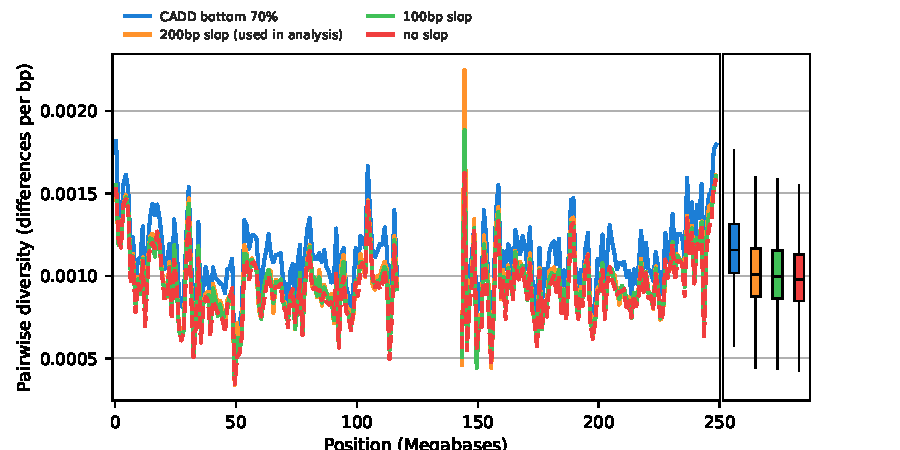
\includegraphics[width=\textwidth]{figures/supplementary/neutral_tracks.pdf}

  \caption{Estimates of chromosome 1 YRI diversity in non-overlapping megabase
      windows, under different neutral tracks (colors) and the filtering
      criteria described in Supplementary Section \ref{supp:accessible}. To the
      right of the chromosome subfigure are the genome-wide boxplots of
      megabase-scale diversity. } 

  \label{suppfig:neutral-tracks}
\end{figure}

Linked selection theory typically assumes that focal sites are not under
purifying selection themselves. Consequently, linked selection statistical
methods often only consider the fraction of the genome not \emph{a priori}
under selective constraint \parencite[e.g. Appendix Section
3.1]{Murphy2022-sj}. Our methods follow suit, and first create a track
consisting of the union (i.e. \texttt{bedtools merge}) of: exons and coding
sequences from Ensembl Version 107
\parencite[\path{Homo_sapiens.GRCh38.107.chr.gff3.gz}]{Cunningham2022-vk} and
PhastCons regions
\parencite[\path{phastConsElements100way.bed.gz}]{Siepel2005-wh}. Then, we
remove 200 basepairs of ``slop" around each of these regions (i.e.
\texttt{bedtools slop}). We show in Supplementary Figure
\ref{suppfig:neutral-tracks} that average diversity (we only consider YRI
samples for this analysis) is fairly insensitive to the slop width, but
increasing slop widths around putatively conserved segments does lead to higher
diversity estimates. This is expected, since increasing the slop width
considers a smaller subset of sites, further away from putatively conserved
regions. For our analyses we choose the 200bp slop version, which covers
63.66\% of the autosomal reference sequence and consists of 1.26 million
contiguous genomic regions.

Additionally, we compared our neutral track (and the slop width alternatives)
against the bottom 70\% of CADD site scores (this works out to be 64.70\% of
the autosomal reference sequence). The correlation between these two tracks is
extraordinarily high (Pearson $r = 0.98$, p-value $=0$), but the average
pairwise diversity is 13\% higher (two-tailed t-test p-value $1.29 \times
10^{-71}$) in the CADD bottom 70\% neutral track. However, we did not use the
CADD bottom 70\%  neutral track in our analysis of human population genomic
data. Our concern was that because CADD models are trained by differentiating
high-frequency derived SNPs in humans from simulated variants at every
basepair, there could be circularity in basing our neutral regions on
predictions based on modeling frequency data. Moreover, this neutral track
would be close to a complement of the CADD 6\% track, which we use as one of
our annotation models, and might lead to issues. Additionally, the CADD bottom
70\% neutral track is much less sparse than the track we used in our analysis,
with a total of $\approx 20$ times more contiguous regions than the neutral
track used in analysis (25.38 million total). Many of these ranges are at very
small spatial scales (average: $\approx 7$ basepairs).

Additionally, we ran one test model with the CADD bottom 70\% as the neutral
track as a test. Using the CADD bottom 70\% neutral track with the CADD 6\%
annotation model, the in-sample was $R^2=63.99$\%; by comparison, the in-sample
$R^2=68.03$\% using the constructed neutral track with 200bp slop. Overall,
future work calibrating the neutral track is needed.

These neutral tracks are all produced by the Snakemake file
\path{data/fit_annotation/Snakefile} in this study's GitHub repository
(\url{http://github.com/vsbuffalo/bprime}). We summarize the percentage of
basepairs after masking per chromosome in Supplementary Table
\ref{supp-table:masks}.

\begin{table}
    \label{supp-table:masks}
\centering
\caption{Accessible and putatively neutral sequence mask statistics, for the criteria used in 
         the main model fits.}
\begin{tabular}{|c|cccc|}
\hline
Chromosome & Accessible (\%) & Neutral (\%) & Intersection (\%) & Total Basepairs ($\times 10^6$) \\
\hline 
1 &        39.7 &     62.0 &  15.7 &     39.09 \\
2 &        45.3 &     60.1 &  18.9 &     45.77 \\
3 &        43.2 &     59.6 &  16.9 &     33.51 \\
4 &        42.7 &     65.9 &  20.2 &     38.42 \\
5 &        42.4 &     62.2 &  18.1 &     32.86 \\
6 &        43.8 &     61.4 &  18.4 &     31.43 \\
7 &        41.9 &     64.0 &  18.6 &     29.64 \\
8 &        42.3 &     66.1 &  20.2 &     29.32 \\
9 &        36.2 &     65.4 &  14.6 &     20.21 \\
10 &        42.9 &     62.2 &  18.8 &     25.15 \\
11 &        41.3 &     61.5 &  17.0 &     22.96 \\
12 &        40.6 &     60.4 &  15.9 &     21.19 \\
13 &        38.8 &     70.7 &  18.8 &     21.50 \\
14 &        36.5 &     64.6 &  13.8 &     14.77 \\
15 &        34.4 &     66.3 &  13.5 &     13.77 \\
16 &        36.0 &     66.0 &  15.5 &     14.00 \\
17 &        37.2 &     58.8 &  14.2 &     11.82 \\
18 &        40.3 &     66.1 &  19.6 &     15.75 \\
19 &        28.1 &     67.5 &  11.5 &      6.74 \\
20 &        36.1 &     62.5 &  15.4 &      9.92 \\
21 &        29.8 &     76.9 &  17.3 &      8.08 \\
22 &        25.5 &     75.5 &  12.6 &      6.40 \\
\hline
weighted average & 40.1 & 63.6 & 17.1 & - \\
\hline
\end{tabular}
\end{table}

\subsection{Window-based Summaries and filtering}

\begin{figure}[!htb]
  \centering
  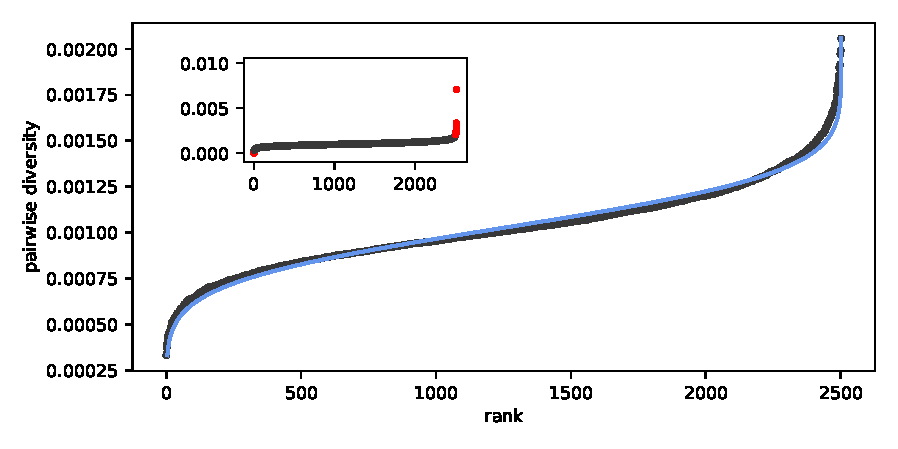
\includegraphics{figures/supplementary/diversity_trimming_dist.pdf}

  \caption{The distribution of diversity across the genome at the megabase
  scale, with outliers trimmed. The blue line is the best-fitting normal CDF.
  We note that this implies the distribution of megabase-scale diversity 
  is slightly fat-tailed compared to a normal distribution.
  The inset figure is the untrimmed data, with trimmed points shown in red. }
  \label{suppfig:trimming}
\end{figure}

Based on exploratory data analyses, we noticed some rare windows that were
outliers. Given that maximum likelihood estimation can be easily biased by
outliers, we took a conservative approach and removed the top 0.5\% of
high-diversity windows. The results of this can be seen in Supplementary
Figure \ref{suppfig:trimming}. We also remove 1cM from each end of the
recombination map. These window-based filters are in addition to the
accessible and neutral sequence masked described in Supplementary Sections
\ref{supp:filter} and \ref{supp:accessible}.

\subsection{Annotation Models}


CADD 6\%: 6.49\% of autosomal sequence.
CADD 8\%: 8.56\% of autosomal sequence.



\subsection{Model Comparisons}

% \begin{table}[ht]
%     \caption{CADD 6\% Sparse Track B and B' Comparison}
%     \label{supptab:cadd6}
%     \centering
% \begin{tabular}{lll}
%                          & \strong{B}              & \strong{B'}                     \\
%                          \hline
%     \emph{negative log-likelihood} & 250,622,462,847.73962     & 250,622,458,048.0578      \\
%     $R^2$                   & 53.89\%                 & 53.9\%                  \\
%     \hline
%     $\pi_0$                 & 0.0014272  & 0.0014297  \\
%     $\mu_\text{del}$        & $1.88 \times 10^{-8}$ & $4.29 \times 10^{-8}$ \\
%     \\
%     \emph{sel. coef.} &\multicolumn{1}{c}{\emph{DFE estimates (percent)}} \\
%     \hline
%     $10^{-8}$                  & 0.0                    & 0.0                    \\
%     $10^{-7}$                   & 0.0                    & 0.0                    \\
%     $10^{-6}$                   & 0.0                    & 0.0                    \\
%     $10^{-5}$                   & 0.3                    & 0.57                   \\
%     $10^{-4}$                  & 10.27                  & 0.02                   \\
%     $10^{-3}$                   & 25.22                  & 0.12                   \\
%     $10^{-2}$                    & 1.91                   & 0.0                    \\
%     $10^{-1}$                     & 62.3                   & 0.28                  \\
%     \hline
% \end{tabular}
% \end{table}

\subsection{Table of $R^2$ Values}

\begin{table}
    \label{supp:tbl-r2}
\centering
\caption{$R^2$ and mutation rate estimates for all models. Note that the repeated values in the last 
rows are correct and due to rounding; see \path{notebooks/main_fits.ipnb} in the GitHub repository for 
more information.}
\begin{tabular}{lll|crr|cc}
    \textbf{Model} & \textbf{Track type} & \textbf{Pop.} & \textbf{B' $R_\text{LOO}^2$} & \textbf{B' $R_\text{IS}^2$} & \textbf{B $R_\text{IS}^2$} & \textbf{B' $\hat{\mu} \times 10^{-8}$} & \textbf{B $\hat{\mu} \times 10^{-8}$} \\[0.5ex] 
\hline
\hline
    \textbf{phastcons$>$CDS$>$genes} &            sparse &          YRI &                        \textbf{68.45} &             68.16 &            65.23 &                                 1.8636 &                                0.2975 \\
phastcons$>$CDS$>$genes &              full &          YRI &                        68.19 &             68.12 &            63.67 &                                 1.7082 &                                0.1666 \\
               CADD 6\% &              full &          YRI &                        68.08 &             68.08 &            62.96 &                                 1.4612 &                                0.1721 \\
               CADD 6\% &            sparse &          YRI &                        68.04 &             68.03 &            68.01 &                                 2.0912 &                                2.0716 \\
               CADD 8\% &              full &          YRI &                        66.98 &             67.11 &            63.61 &                                 1.0126 &                                0.1713 \\
               CADD 8\% &            sparse &          YRI &                        66.67 &             67.01 &            66.98 &                                 1.5688 &                                1.5473 \\
CDS$>$genes$>$phastcons &              full &          YRI &                        64.90 &             65.51 &            61.23 &                                 4.1951 &                                0.1620 \\
CDS$>$genes$>$phastcons &            sparse &          YRI &                        64.90 &             65.51 &            63.16 &                                 4.1795 &                                0.3070 \\
\textbf{phastcons$>$CDS$>$genes} &            sparse &          CEU &                        \textbf{61.98} &             63.02 &            60.02 &                                 2.0194 &                                0.3036 \\
phastcons$>$CDS$>$genes &              full &          CEU &                        61.78 &             63.01 &            58.57 &                                 2.3499 &                                0.1679 \\
               CADD 6\% &              full &          CEU &                        61.74 &             62.94 &            57.42 &                                 1.5365 &                                0.1739 \\
               CADD 6\% &            sparse &          CEU &                        61.66 &             62.86 &            62.84 &                                 2.1215 &                                2.1084 \\
               CADD 8\% &              full &          CEU &                        60.80 &             62.12 &            57.95 &                                 1.1572 &                                0.1742 \\
               CADD 8\% &            sparse &          CEU &                        60.59 &             62.06 &            62.04 &                                 1.6030 &                                1.5876 \\
               CADD 6\% &              full &          CHB &                        59.62 &             61.31 &            55.31 &                                 1.5083 &                                0.1727 \\
               CADD 6\% &            sparse &          CHB &                        59.54 &             61.21 &            61.20 &                                 2.1242 &                                2.1170 \\
               \textbf{phastcons$>$CDS$>$genes} &            sparse &          CHB &                        \textbf{59.44} &             61.08 &            57.88 &                                 2.1982 &                                0.3060 \\
phastcons$>$CDS$>$genes &              full &          CHB &                        59.29 &             61.08 &            56.71 &                                 2.5573 &                                0.1694 \\
               CADD 8\% &              full &          CHB &                        58.88 &             60.63 &            55.86 &                                 1.1128 &                                0.1733 \\
               CADD 8\% &            sparse &          CHB &                        58.65 &             60.57 &            60.55 &                                 1.6098 &                                1.6001 \\
CDS$>$genes$>$phastcons &            sparse &          CEU &                        58.58 &             60.30 &            58.41 &                                 4.1041 &                                0.3110 \\
CDS$>$genes$>$phastcons &              full &          CEU &                        58.58 &             60.30 &            56.75 &                                 4.1001 &                                0.1648 \\
CDS$>$genes$>$phastcons &            sparse &          CHB &                        56.48 &             58.73 &            56.60 &                                 3.7195 &                                0.3136 \\
CDS$>$genes$>$phastcons &              full &          CHB &                        56.48 &             58.73 &            54.95 &                                 3.7552 &                                0.1654 \\
\hline
\end{tabular}
\end{table}


\subsection{Derivation of Approximate Coalescence $R_\text{coal}^2$}
\label{supp:r2-coal}

Our approach models the observed megabase-scale diversity $y_i$ in window $i$
as the predicted level under our negative selection model, $\pi_0 B_i$, plus
some random residual error $\varepsilon_i$,

\begin{align}
    y_i = \pi_0 B_i + \varepsilon_i
\end{align}

where each $B_i = f(X_i | \Psi)$ for some data $X_i$ (i.e. the recombinaton map
and annotation model) and parameters $\Psi$. To compare our models and assess
model goodness-of-fit, we use the out-sample $R_\text{LOO}^2$ which is
calculated by fitting the genome-wide model leaving one chromosome out, and
calculating the residual variance between predictions and observed values for
this out-sample chromosome. 

In general, $R^2$ is calculated for a model fit across windows as,

\begin{align}
    R^2 = 1 - \frac{V_\text{res}}{V_\text{tot}}
\end{align}

where $V_\text{res}$ is the mean squared error across windows and
$V_\text{tot}$ is the total variance in the observed values. Suppose we have
estimates $\widehat{\pi}_0 \widehat{B}_i$ for $\pi_0 B_i$ from our model. Then,

\begin{align}
    V_\text{res} &= \frac{1}{n} \sum_{i=1}^n (y_i - \widehat{\pi}_0 \widehat{B}_i)^2  \\
                 &= \underbrace{\frac{1}{n} \sum_{i=1}^n \varepsilon_i^2}_\text{irreducible error} + \underbrace{\left(\frac{1}{n} \sum_{i=1}^n (\pi_0 B_i - \widehat{\pi}_0 \widehat{B}_i)\right)^2}_\text{bias squared}.
\end{align}

The total variance among the observed diversity values is,

\begin{align}
    V_\text{tot} = V_\text{res} + V_\text{model} + 2\widehat{\pi}_0\cov_i(\varepsilon_i, \widehat{B}_i)
\end{align}
where 
\begin{align}
    V_\text{model} = \frac{\widehat{\pi}_0^2}{n} \sum_{i=1}^n \left(\widehat{B}_i - \frac{1}{n}\sum_{i=1}^n\widehat{B}_i\right)^2.
\end{align}

Generally, fitting procedures act to minimize the squared deviation between
predictors and observed values, which drives $\cov_i(\varepsilon_i,
\widehat{B}_i)$ to zero XXX. \textcite{Murphy2022-sj} suggest  XXX 

Thus, our $R^2$ depends on (1) the bias of our predictors, (2) the covariance
between residuals and predictors, and (3) the irreducible error due to variance
in diversity within windows. However, it is of interest to approximate the
irreducible error under theoretic models that assume all irreducible error is
due entirely to the variance of coalescence times in a window, assuming that
all of the effects of negative selection on the variance can be thought of as a
local reduction in the effective population size to $B_i N_e$ and demographic
effects amount to a simple rescaling of $N_e$. This also assumes mutation rates
are constant across the genome, and do not contribute to the irreducible
variance. We call this theoretic goodness-of-fit under drift
$R_\text{drift}^2$, and it provides a rough approximation of the irreducible
error in our model due to ``coalescence noise" around the modeled reductions
due to negative selection.

Then, 

\begin{align}
    \E(\varepsilon_i^2) = \V(\pi_i)
\end{align}

since the mean residual is zero. The variance in pairwise diversity
$\V(\pi_i)$ is equivalent to the variance in the number of segregating sites
for a sample of two, $\V(\pi) = \V(S_2)$. The variance in coalescence times
in a window of width $w$ basepairs with population-scaled recombination rate
$\rho = 4 B_i N_e r w$ is,

\begin{align}
    \V(S_2) = \theta + \theta^2 \frac{2}{\rho^2} \int_0^\rho (\rho - x) f_2(x) dx
\end{align}
(\cite[eq. 7.20]{Wakeley2009-ua}) where,
\begin{align}
    f_2(\rho) = \frac{\rho + 18}{\rho^2 + 13 \rho + 18}.
\end{align}

Since this is a rough approximation,  we set $\theta = w \pi_0 B_i$ and fix
$\rho = w \gamma \pi_0 B_i$ where $\gamma$ is the ratio of recombination to
mutation rates, $\nicefrac{r}{\mu}$. In humans, $\gamma \approx 1$, but we
explore different ratios to assess sensitivity of this calculation
(Supplementary Figure \ref{suppfig:r2_upper}). 

This back-of-the-envelope calculation finds that the upper bound of $R^2$ would
be around 67\% for Yoruba, and 64\% for European and Han Chinese models (Figure
\ref{suppfig:drift_r2} This rough approximation assumes constant demography,
which for bottlenecked out-of-Africa populations assumes that the variance in
coalescence times is determined entirely by reducing the effective population
size. However, the variance in coalescence times is \emph{higher} in
bottlenecked populations (CEU and CHB) compared to Yoruba, which we confirm
with simple simulations using the \texttt{OutOfAfrica\_3G09} model from
\texttt{stdpopsim} \parencite{Gutenkunst2009-pg,Adrion2020-cf}. This higher
than expected variance would inflate $SS_\text{res}$, which would decrease
$R_\text{drift}^2$, bringing it closer to the observed $R_\text{LOO}^2$. A more
accurate approximation of the $R_\text{drift}^2$ could be found with
simulations with more realistic demography and varying coalescence rates along
the genome.

\begin{figure}[htbp] \centering
    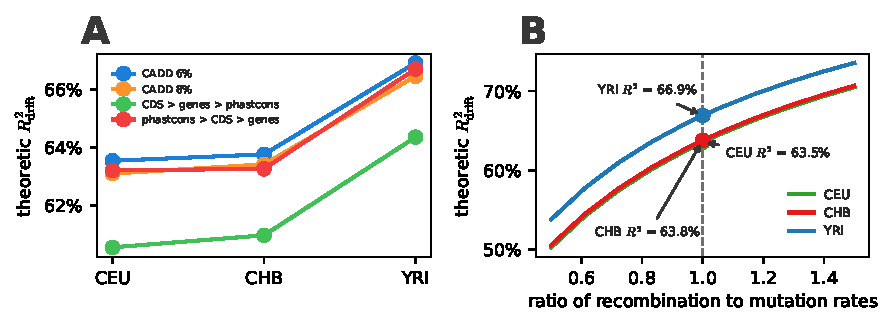
\includegraphics[width=\textwidth]{figures/supplementary/suppfigure_drift_R2.pdf}
    \caption{(A) the theoretic $R_\text{drift}^2$ using different plugin
        estimators for $B_i$ under different models. This shows that among the
        best-fitting models, the predicted $R_\text{drift}^2$ varies little;
        most variation is among populations due to differing $\pi_0$. (B) The 
        $R_\text{drift}^2$ across different populations, for varying ratio of recombination
        to mutation rates (x-axis).}
  \label{suppfig:drift_r2}
\end{figure}

\subsection{Predicted Rate of Fitness Change}

Each fixation of a mutant with fitness effect $-s$ reduces the population
fitness to $1-2s$ since all individuals are homozygotes for the deleterious
mutation and we assume additive effects at a site. For each segment $l$, the
maximum likelihood parameter estimates of our model imply a prediction of the
deleterious substitution rate per segment $\widehat{R}_{l,i}$ for each
selection coefficient $s_i$ in the $m_s$-element DFE grid (according to which
feature class it belongs to).

Since we assume multiplicative fitness effects, the log population fitness
(considering only fixed sites) for segment $l$ in the next generation is,

\begin{align}
    \log(L_{l}) = \sum_{i=1}^{m_s} \log(1-2 s_i) \widehat{R}_{l,i}.
\end{align}
%
Since we assume multiplicative fitness, the total genome-wide log population
fitness in the next generation is

\begin{align}
    \log(L) = \sum_{l} \log{L_l}.
\end{align}
%
This amounts to a predicted population fitness loss per generation of

\begin{align}
    \widehat{\Delta}_W &= 1 - L \\  \nonumber
             &= 1 - \exp\left(\sum_{l} \sum_{i=1}^{m_s} \log(1-2s_i) \widehat{R}_{l,i} \right).
\end{align}
%
We calculate this value for all segments within a feature class, and then sum
over all features to arrive at our genome-wide estimate. We use a parametric
bootstrap to carry forward the estimation uncertainty to the predicted fitness
loss per generation. Briefly, we do this by sampling new estimates of the DFE
per selection coefficient and feature from a normal distribution centered on
the ML point estimate and with the jackknife standard deviation.

\subsection{Likelihood}
\label{supp:likelihood}

Our model is essentially a generalized nonlinear model with a binomial link
function. This is the form used by \textcite{Elyashiv2016-vt} and
\textcite{Murphy2022-sj}. These models fit the observed number of pairwise
nucleotide differences in genomic windows to the expected pairwise diversity
under some evolutionary model. We only consider BGS models here, so the mean
function for position $x$ is the product of the proportion by which BGS reduces
diversity at position $x$, $B(x)$, and genome-wide neutral diversity $\pi_0$,

\begin{align}
  \pi(x) = B(x, \Phi) \pi_0
\end{align}

$\Phi$ is the set of BGS parameters (i.e. the DFE matrix $\mathbf{W}$ and
mutation rate $\mu$), and $\pi_0 = 4 N_e \mu$ is determined by the genome-wide
drift-effective population size $N_e$, set by only reproductive and demographic
processes. Regional mutation rate heterogeneity can be accounted for with a
regional mutation rate scaling function $m(x)$, $\pi(x) = B(x, \Phi) m(x)
\pi_0$, but we do not explore mutation-rate heterogeneity, as it is unclear how
to differentiate variance in mutation rate from the substitution rate
heterogeneity we find across the genome.

The likelihood of the set of parameters $\Psi = \{\pi_0, \Phi\}$ can be written
in the form of, 

\begin{align}
  \log\mathcal{L}(\Psi) = \sum_{v \in \mathcal{V}} \sum_{i \ne j \in \mathcal{S}} \log(P(O_{i,j}(v) | \Psi))
\end{align}

(c.f. \cite{McVicker2009-ax,Elyashiv2016-vt,Murphy2022-sj}) where $\mathcal{V}$
is the set of putatively neutral sites, $\mathcal{S}$ is the set of samples,
and $\Psi$ are the BGS parameters. The indicator variable $O_{i,j}(v)$ is 1 if
samples $i$ and $j$ are different at putatively neutral site $v$, and zero
otherwise. While the theoretic $\pi(v)$ gives the average number of pairwise
differences, for small values, this is approximately the heterozygosity
probability, so we can write

\begin{align}
  P(O_{i,j}(v) | \Psi) = 
    \begin{cases}
      \pi(v), & O_{i,j}(v, \Psi) = 1 \\
      1-\pi(v), & O_{i,j}(v, \Psi) = 0 \\
    \end{cases}.
\end{align}

(c.f. \cite{Elyashiv2016-vt}). 

As in Section \ref{supp:diversity}, the number of pairwise differences and
the total number of pairwise comparison at a site are sufficient statistics for
the likelihood. Then, the binomial log-likelihood for the data at site $v$ is,

\begin{align}
  \ell_v(\Psi) &= \log(\pi(v, \Psi)) n_{\text{D},v} + \log(1-\pi(v, \Psi)) n_{\text{S},{v}}
\end{align}

\subsection{The scale of processes}

We can observe $\widehat{\pi}(x)$ at a per-basepair resolution. However, for a
variety of reasons, we do not want to fit the composite likelihood model to the
per-basepair scale of data. First, this would be computationally infeasible.
Second, the mean function $\pi(x)$ varies on a natural scale that is itself a
free parameter of the model. Our model can be written as, 

\begin{align}
  \ell(\Psi, h) &= \sum_{b} \sum_{v \in \mathcal{V}_b} \ell_v(\Psi) \\
             &= \sum_{b} \left[\log(\bar{\pi}(b, \Psi)) \sum_{v \in \mathcal{V}_b} n_{\text{D},v} + \log(1-\bar{\pi}(b, \Psi)) \sum_{v \in \mathcal{V}_b} n_{\text{S},{v}}\right] \\
             &= \sum_{b} \left[\log(\bar{\pi}(b, \Psi)) Y_{\text{D},b} + \log(1-\bar{\pi}(b, \Psi)) Y_{\text{S},{b}}\right] \\
\end{align}

where $h$ is the bandwidth or window size, $b$ the bin index for windows of
width $h$, $\mathcal{V}_b$ is the set of putatively neutral sites in bin $b$,
$\bar{\pi}(b | \Psi)$ are the average diversity in bin $b$, and
$Y_{\text{S},b}$ and $Y_{\text{S},b}$ are the sums across putatively neutral
sites within a bin. Note that by binning, we sum the pairwise summaries of the
data $\mathbf{Y}$ across sites, so the likelihood across bins is naturally
weighted by the quantity of observed data. 


% TODO
%We estimate $h$ by fitting the model
%for a variety of window sizes $h$ and select the best using out-sample cross
%validation, as is standard in non-parametric regression (XXX, Wasserman, p.
%70).

This model corresponds to a binomial likelihood for the observed data
summarized at genomic scale $h$. Thus an alternative way to express this model
is as, 

\begin{align}
  Y_{\text{D},b} \sim \text{Binom}(\bar{\pi}(b, \Psi), Y_{\text{D},b} + Y_{\text{S},b}).
\end{align}

Here, $\bar{\pi}(b, \Psi)$ is assumed to be the \emph{probability} of sampling
two different alleles, rather than the average \emph{number} of pairwise
differences; these are approximately equal when $\pi$ is small. This
corresponds to an identity link function; one could alternatively use a
two-alleles finite sites model link function of the form, $\pi/(1 + 2 \pi)$. We
experimented with this and found there was little difference between these link
functions, so we opted for the simpler identity link function.

\subsection{Out-Sample Error Estimation and $\widehat{R}_\text{LOCO}^2$}

To estimate out-sample prediction error, we fit each model leaving one
chromosome out (LOCO) and calculating the out-sample prediction error on
these excluded chromosomes. Each fit used 10,000 random starting positions as
the main fits. The out-sample prediction error (i.e. sum of residuals
squared, $\widehat{\mathrm{SSR}}_\text{LOCO}$) for all bins in chromosome $C$
left out is,

\begin{align}
    \widehat{\mathrm{SSR}}_\text{LOCO}(C) = \sum_{b \in C} (\widehat{\pi}_{b, (C)}  - \pi_b)^2
\end{align}
%
where $\widehat{\pi}_{b,(C)}$ denotes the predictions for window $b$ fit on
data excluding chromosome $C$. The average out-sample error
$\widehat{\mathrm{SSR}}_\text{LOCO}$ across chromosomes is then the average of
$\widehat{\mathrm{SSR}}_\text{LOCO}(C)$ across chromosomes, weighted by the
number of bins per chromosome. We then calculate the out-sample coefficient of
determination $\widehat{R}_\text{LOCO}^2$

\begin{align}
    \widehat{R}_\text{LOCO}^2 = 1-\frac{\widehat{\mathrm{SSR}}_\text{LOCO}}{\widehat{\mathrm{SST}}_\text{LOCO}}
\end{align}
%
where, 

\begin{align}
    \widehat{\mathrm{SST}}_\text{LOCO}(C) = \sum_{b \in C} (\widehat{\pi}_{b, (C)}  - \bar{\pi})^2
\end{align}
%
and $\bar{\pi}$ is the average diversity across all windows.

\subsection{Jackknife Procedures}
\label{supp:jackknife}

\begin{figure}[htbp]
  \label{suppfig:jackknife-iqr}
  \centering
  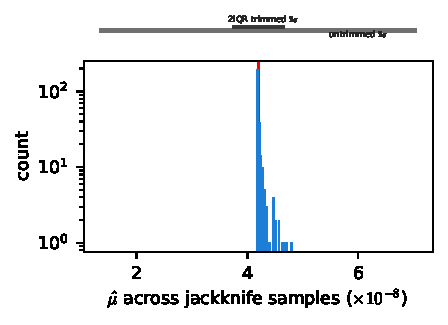
\includegraphics[width=0.7\textwidth]{figures/supplementary/iqr_jackknife_trim.pdf}

  \caption{The distribution of block jackknife samples for the Feature Priority
  model fit on YRI data. The ranges at the top of the figure indicate the
untrimmed and the 2 IQR-trimmed jackknife intervals. for XXX fix fig }

\end{figure}

We use a block jackknife procedure to calculate the uncertainty of our
estimates. This approach is unfortunately computationally intensive, since a
10Mbp block width requires $\approx 280$ blocks to cover 2.8Gbp of autosomal
sequence and each fit requires thousands of random starts to reliably find
consistent optima. We use a parallelization strategy where a set number of
evenly-spaced positions along the genome that are chosen to approximately cover
all 2.8Gbps of autosomal sequence. Each of these positions is sent out across a
computing cluster, which excludes the 10Mbp block there and fits on the
remaining data. Then, using these jackknife samples we calculated the jackknife
standard error for each of parameters \parencite{Wasserman2004-ip}. In some
cases, our jackknife standard error estimates were very large. Upon inspection
of optimization diagnostic plots (see Supplementary Materials Section
\ref{suppfig:diag-plot}) and histograms of jackknife fits (Supplementary Figure
\ref{suppfig:jackknife-iqr}), these were due to rare aberrant optima. We
removed these using a trimmed-interquartile range, which removes points that
are 2 interquartile ranges below the first quartile or above the third quartile
(1.5 is standard, but we chose to be more conservative to not underestimate
uncertainty).

\section{Simulations}
\label{supp:simulation}

All of our forward simulations used SLiM version 4.0.1
\parencite{Haller2019-vu,Haller2023-uk} and all Eidos scripts are available in
the \path{slim_sims/} directory in the GitHub repository
(\url{https://github.com/vsbuffalo/bprime}). These Eidos scripts take command
line arguments for the parameters. Our simulation pipelines use YAML
configuration files that specify the parameter grids and other settings, which
are read and dispatched across a cluster using Snakemake
\parencite{Koster2012-iv}.

\subsection{Segment Simulations}

To confirm the SC16 theory, we simulated a 100 kbp segment in a population of
$N=1000$ diploids across grids of mutation and selection parameters. The Eidos
script for these simulations can be found at
\path{slim_sims/region/region.slim} and the analysis notebook at
\path{notebooks/region_simulations.ipynb} in the GitHub repository
(\url{https://github.com/vsbuffalo/bprime}). We simulated over grids of
mutation rates ($\mu \in \{10^{-9.5}, 10^{-9}, 10^{-8.5}, 10^{-8}\}$) and
selection coefficients ($s \in \{10^{-1}, 10^{-1.5}, 10^{-2}, \ldots,
10^{-4.5}\}$). Selection was additive within a site and multiplicative across
sites, and recombination was fixed at $10^{-8}$ per basepair.


We replicated $10,000$ simulations for each parameter combination to average
and compare against theory. Each simulation recorded the number of fixations
and the fitness variance per generation. At the end $10N$ generations, the
ancestral recombination graph was recorded. Then, downstream Python scripts
calculate branch-length diversity using \texttt{tskit}
\parencite{Kelleher2018-qu}, and we estimate the reduction factor in a window
centered in the region with $B = \nicefrac{\pi}{4N}$ (since branch length
diversity implies $\mu=1$).

\subsection{Whole-chromosome Simulations}

Our whole-chromosome simulations use realistic human recombination maps and
putatively conserved segments. These annotation differ slightly from our
primary model fits, since these simulations were written before the method was
finalized. We use the HapMap recombination map
\parencite{International_HapMap_Consortium2007-nu}, PhastCons regions, and UTRs
as an approximate set of putatively conserved segments. 

Our first set of simulations were used to validate that our methods were
producing accurate classic B and B' maps. We replicated $100$ whole-chromosome
simulations over grids of mutation rates ($\mu \in \{10^{-10}, 10^{-9.5},
\ldots, 10^{-8}, 10^{-7.5}\}$) and selection coefficients ($s \in \{10^{-1},
10^{-1.5}, 10^{-2}, \ldots, 10^{-6}\}$). For each parameter combination, we
calculate mean branch diversity in 10 kbp windows across the 100 replicates to
create the average simulation reduction map. 

We then compare this average simulation map to our method's theoretic B' maps
(see Figure \ref{fig:figure-1} D and E). We calculate the MSE per 10 kbp window
to estimate the total rate across the chromosome. We can assess the accuracy
relative to a theoretic lower bound of the MSE if the noise were due to
coalescence noise. We approximate this by noting that the MSE can be decomposed
into a squared bias term and a variance term. If our methods are unbiased in
estimating the true reduction at a position, the MSE is just the stochastic
variance due to the $n=100$ replicates we simulate and the coalescence noise in
each one. \textcite{Tajima1983-gu} showed that variance in diversity due to
coalescence noise is much larger than sampling noise, and is given by
$\var(\pi) \approx \nicefrac{2\theta^2}{9}$ in an infinite sample. One can
derive an analogous equation for the variance of average simulation $\bar{B}$
across $n$ replicate simulations as, $\var(\bar{B}) \approx
\nicefrac{2B^2}{9n}$. We note that this assumes no recombination but this
approximation is fine over short scales (such as the 10 kbp scale used here).

\section{Additional Results and Figures}

\subsection{Optimization and Diagnostics}
\label{supp:optim}

We only show one optimization diagnostic plot here (Supplementary Figure
\ref{suppfig:diag-plot}), but the can be easily calculated from the model
pickle files in the XXX repository (XXX). In one case, our optimization
diagnostics indicated that the best optima across 10,000 random starts was one
of few of the top 100 hits that were hitting either an alternate likelihood
mode, or the optimization routine had numeric issues. In this one case, we
removed the top hit and used the second, which was the consensus among the
other top 100 optima. 

\begin{figure}[htbp]
  \label{suppfig:diag-plot}
  \centering
  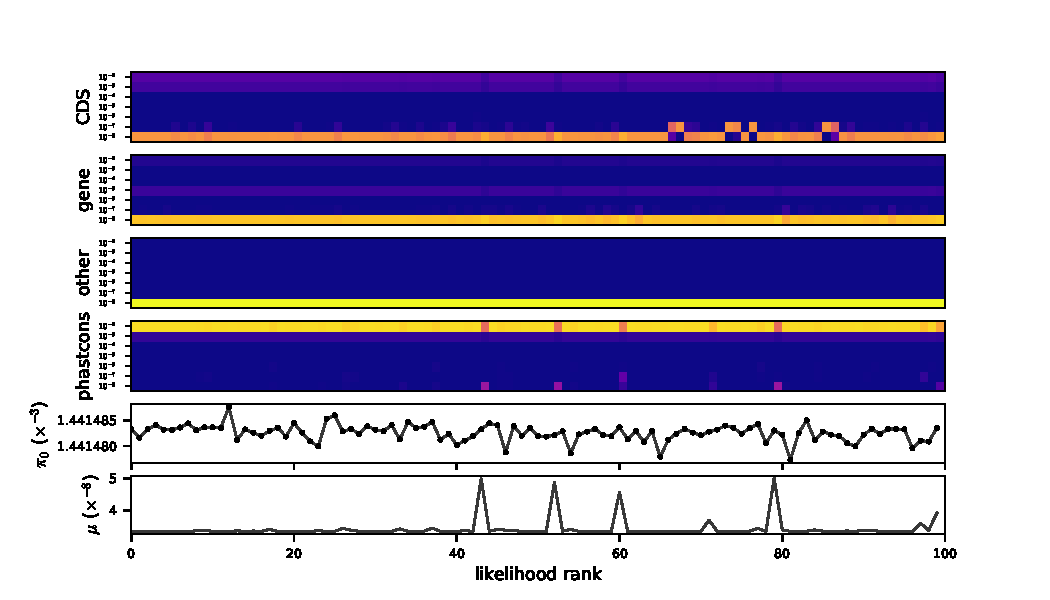
\includegraphics[width=\textwidth]{figures/supplementary/figure_feature_priority_yri_full_diag.pdf}

  \caption{ An optimization diagnostic plot showing the 100 top optima. Heatmap
  colors indicate probability mass for the DFE parameters (top four rows).
Estimates of $\pi_0$ and $\mu$ are shown in the bottom two rows. This is the
optimization plot for YRI Feature Priority model.}
\end{figure}

\clearpage

\subsection{Chromosome Fit Figures}

\begin{figure}[!htb]
  \centering
  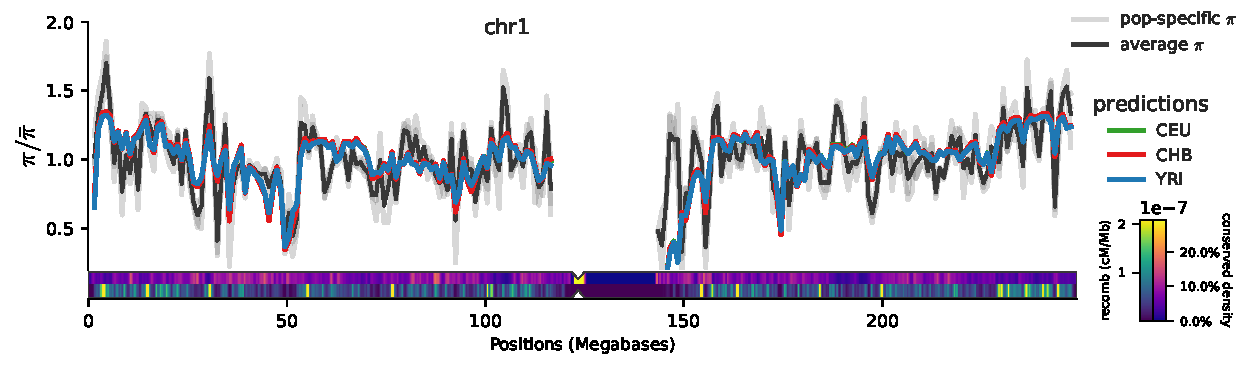
\includegraphics[width=\textwidth]{figures/supplementary/pred_plot_chr1.pdf}
  \label{suppfig:fit-chr1}
\end{figure}

\begin{figure}[!htb]
  \centering
  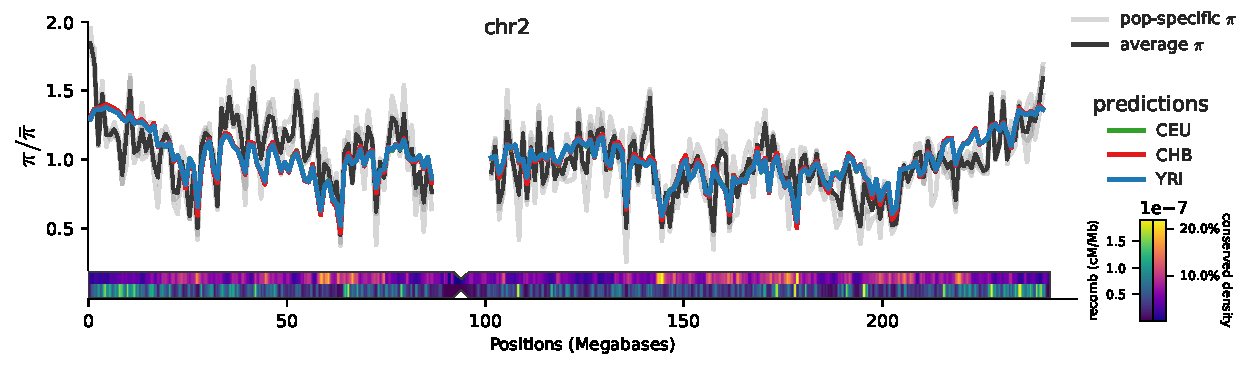
\includegraphics[width=\textwidth]{figures/supplementary/pred_plot_chr2.pdf}
  \label{suppfig:fit-chr2}
\end{figure}


\begin{figure}[!htb]
  \centering
  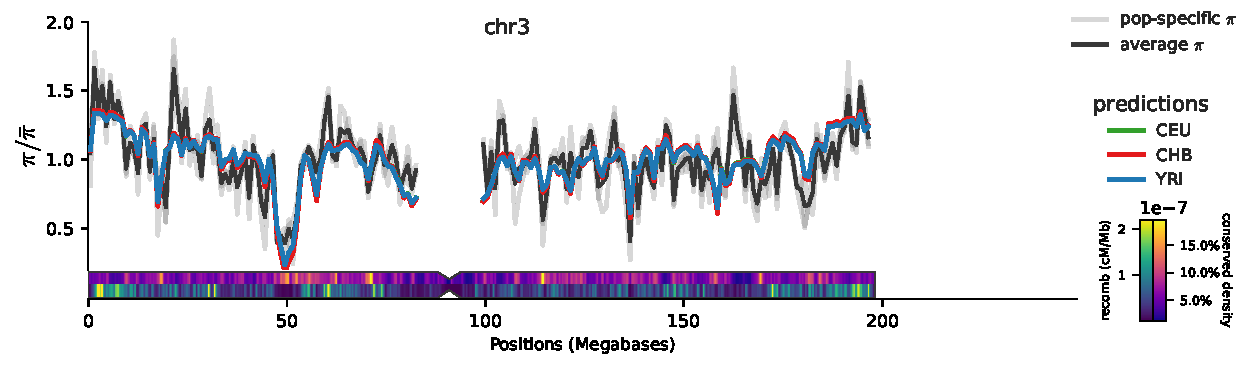
\includegraphics[width=\textwidth]{figures/supplementary/pred_plot_chr3.pdf}
  \label{suppfig:fit-chr3}
\end{figure}


\begin{figure}[!htb]
  \centering
  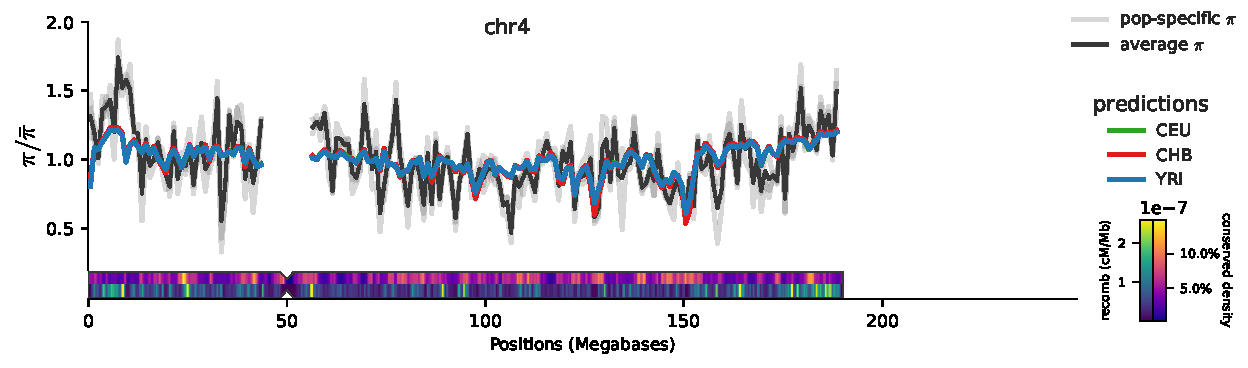
\includegraphics[width=\textwidth]{figures/supplementary/pred_plot_chr4.pdf}
  \label{suppfig:fit-chr4}
\end{figure}


\begin{figure}[!htb]
  \centering
  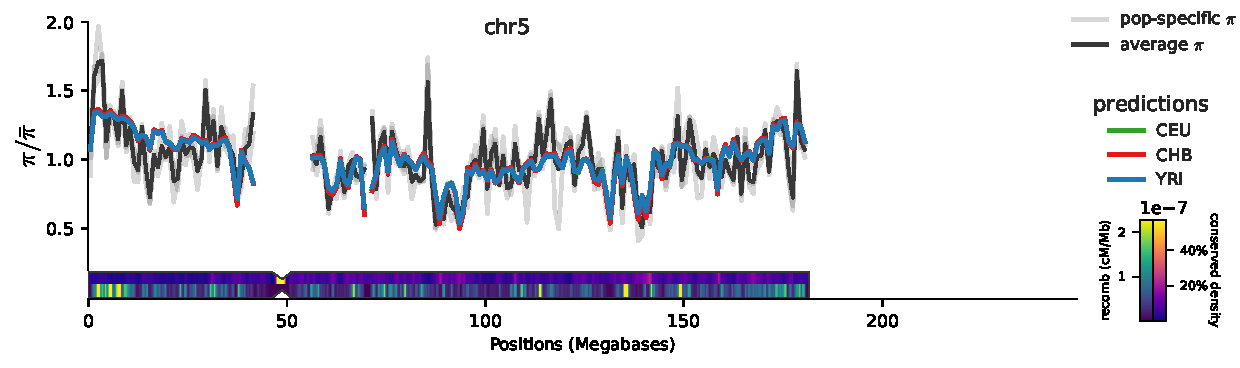
\includegraphics[width=\textwidth]{figures/supplementary/pred_plot_chr5.pdf}
  \label{suppfig:fit-chr5}
\end{figure}


\begin{figure}[!htb]
  \centering
  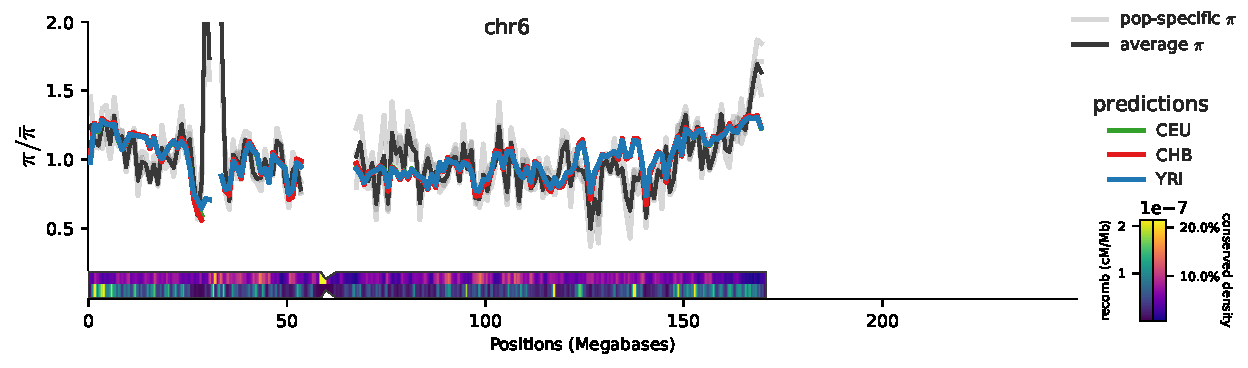
\includegraphics[width=\textwidth]{figures/supplementary/pred_plot_chr6.pdf}
  \caption{Note: we mask the MHC region during model fit.}
  \label{suppfig:fit-chr6}
\end{figure}


\begin{figure}[!htb]
  \centering
  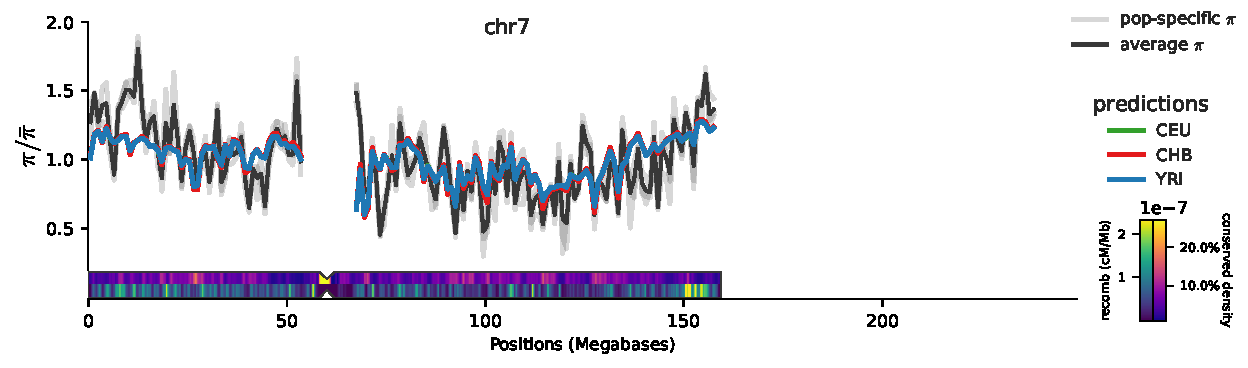
\includegraphics[width=\textwidth]{figures/supplementary/pred_plot_chr7.pdf}
  \label{suppfig:fit-chr7}
\end{figure}


\begin{figure}[!htb]
  \centering
  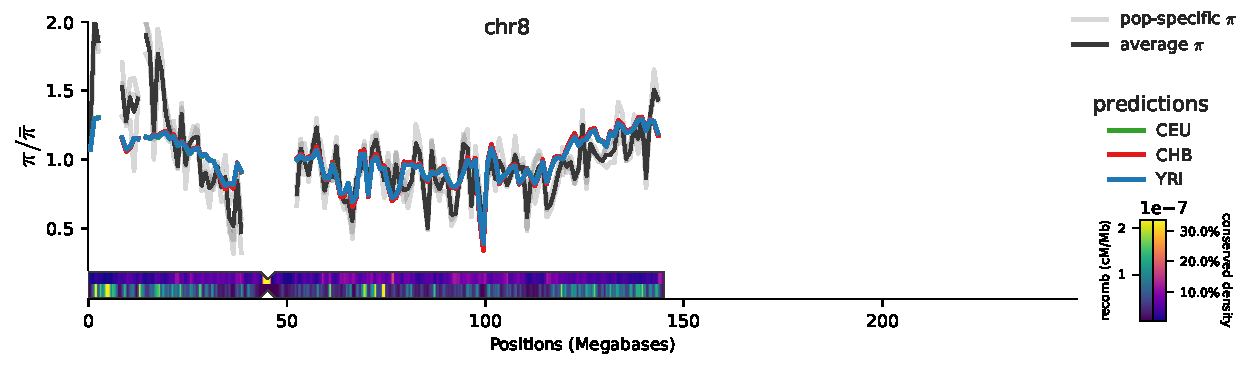
\includegraphics[width=\textwidth]{figures/supplementary/pred_plot_chr8.pdf}
  \label{suppfig:fit-chr8}
\end{figure}


\begin{figure}[!htb]
  \centering
  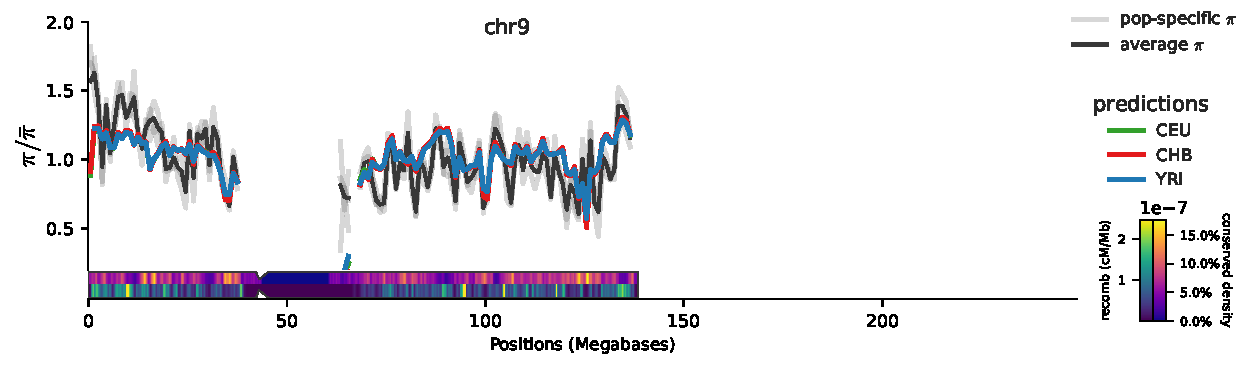
\includegraphics[width=\textwidth]{figures/supplementary/pred_plot_chr9.pdf}
  \label{suppfig:fit-chr9}
\end{figure}


\begin{figure}[!htb]
  \centering
  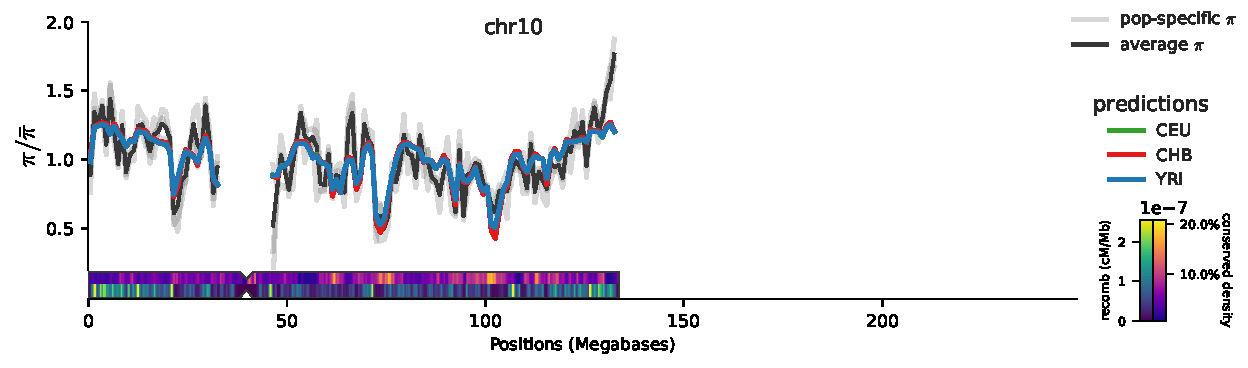
\includegraphics[width=\textwidth]{figures/supplementary/pred_plot_chr10.pdf}
  \label{suppfig:fit-chr10}
\end{figure}


\begin{figure}[!htb]
  \centering
  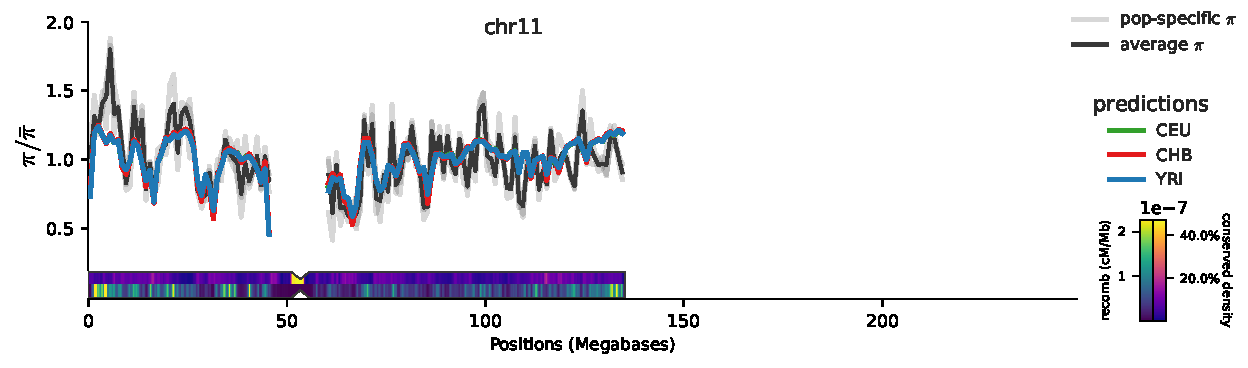
\includegraphics[width=\textwidth]{figures/supplementary/pred_plot_chr11.pdf}
  \label{suppfig:fit-chr11}
\end{figure}


\begin{figure}[!htb]
  \centering
  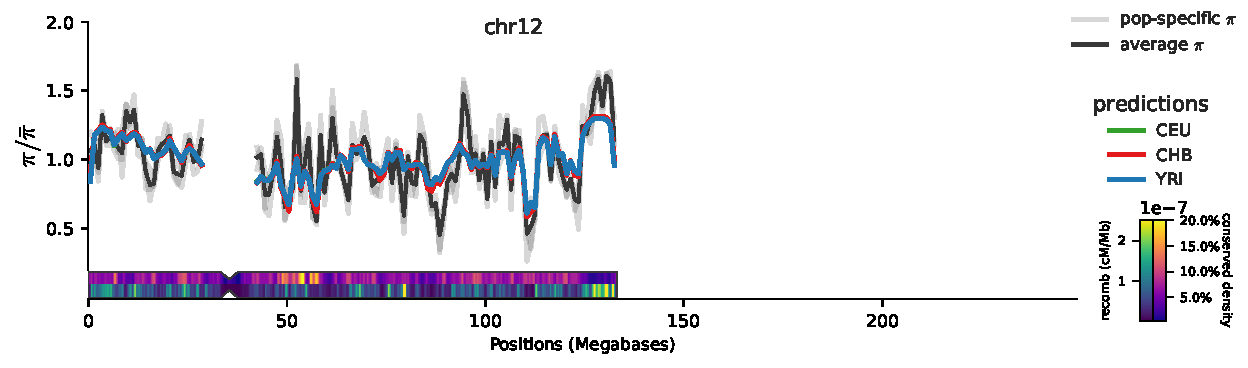
\includegraphics[width=\textwidth]{figures/supplementary/pred_plot_chr12.pdf}
  \label{suppfig:fit-chr12}
\end{figure}


\begin{figure}[!htb]
  \centering
  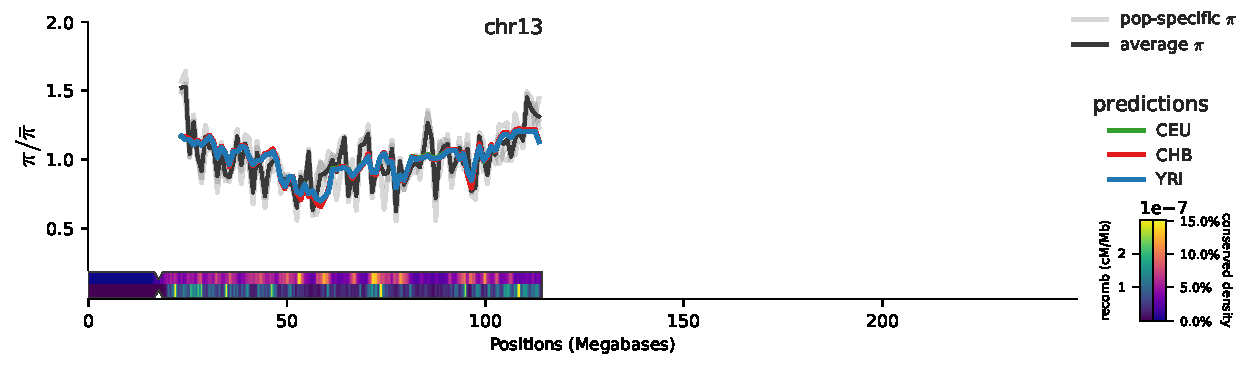
\includegraphics[width=\textwidth]{figures/supplementary/pred_plot_chr13.pdf}
  \label{suppfig:fit-chr13}
\end{figure}


\begin{figure}[!htb]
  \centering
  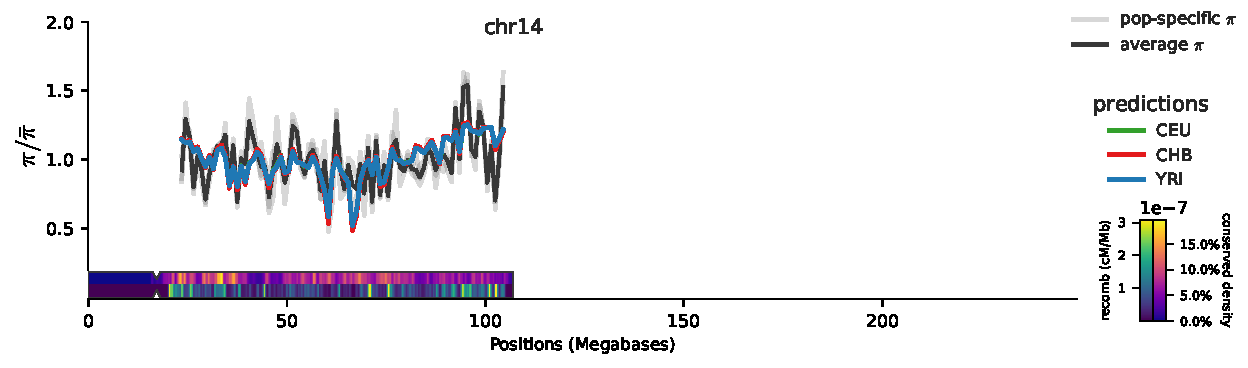
\includegraphics[width=\textwidth]{figures/supplementary/pred_plot_chr14.pdf}
  \label{suppfig:fit-chr14}
\end{figure}


\begin{figure}[!htb]
  \centering
  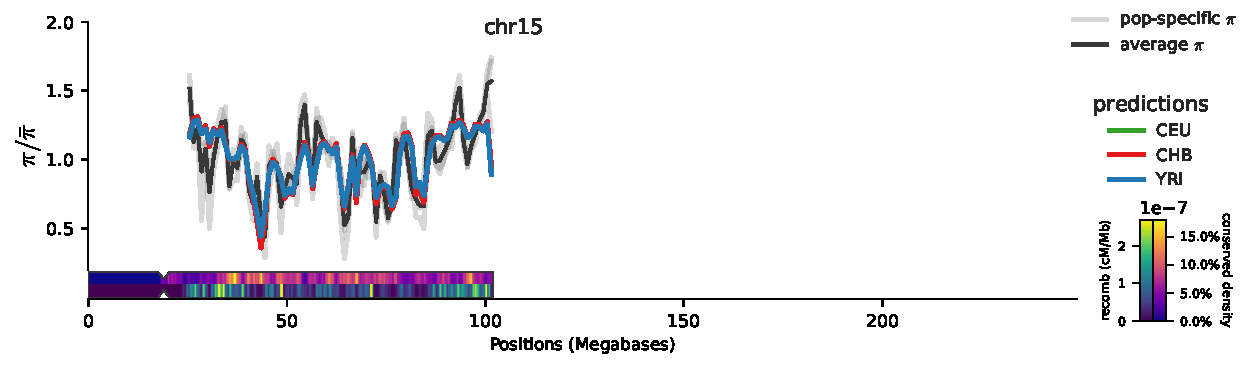
\includegraphics[width=\textwidth]{figures/supplementary/pred_plot_chr15.pdf}
  \label{suppfig:fit-chr15}
\end{figure}


\begin{figure}[!htb]
  \centering
  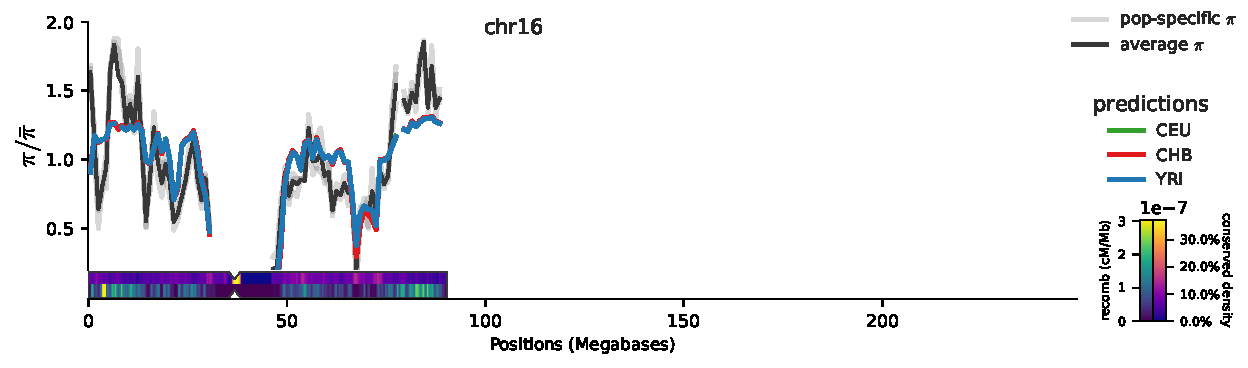
\includegraphics[width=\textwidth]{figures/supplementary/pred_plot_chr16.pdf}
  \label{suppfig:fit-chr16}
\end{figure}


\begin{figure}[!htb]
  \centering
  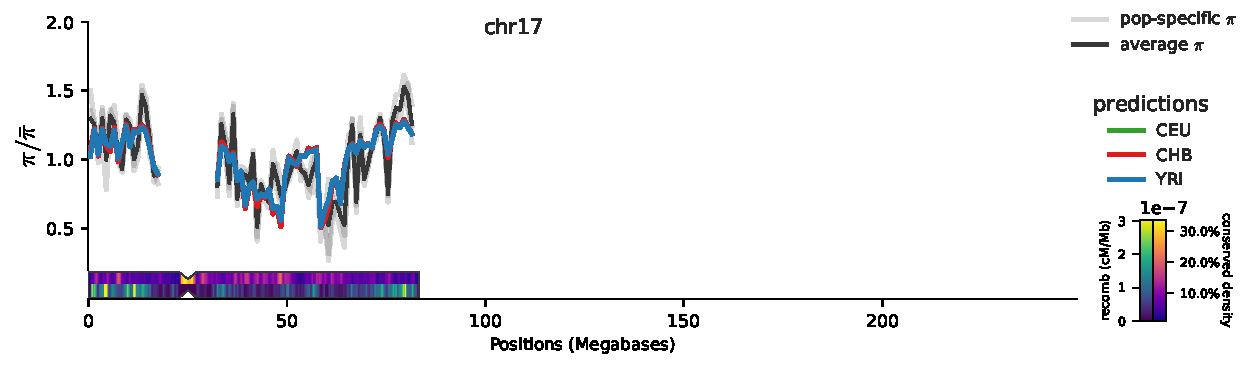
\includegraphics[width=\textwidth]{figures/supplementary/pred_plot_chr17.pdf}
  \label{suppfig:fit-chr17}
\end{figure}


\begin{figure}[!htb]
  \centering
  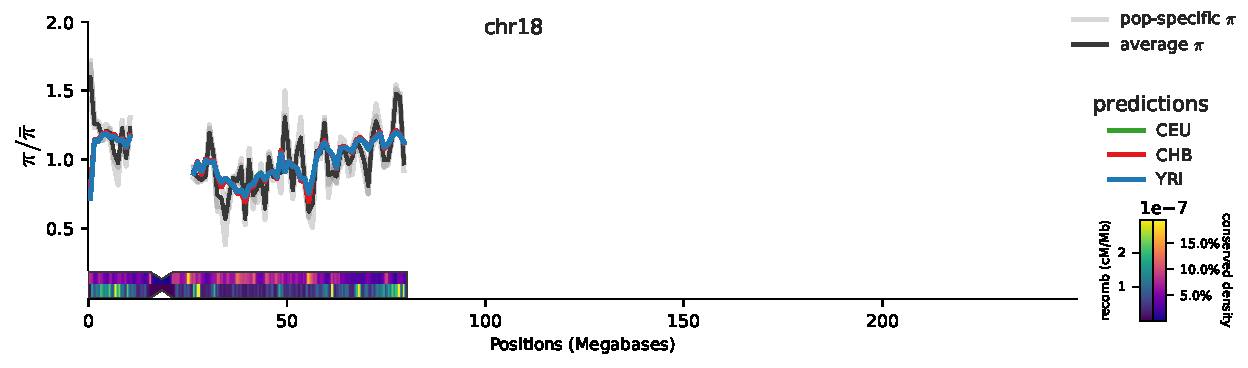
\includegraphics[width=\textwidth]{figures/supplementary/pred_plot_chr18.pdf}
  \label{suppfig:fit-chr18}
\end{figure}


\begin{figure}[!htb]
  \centering
  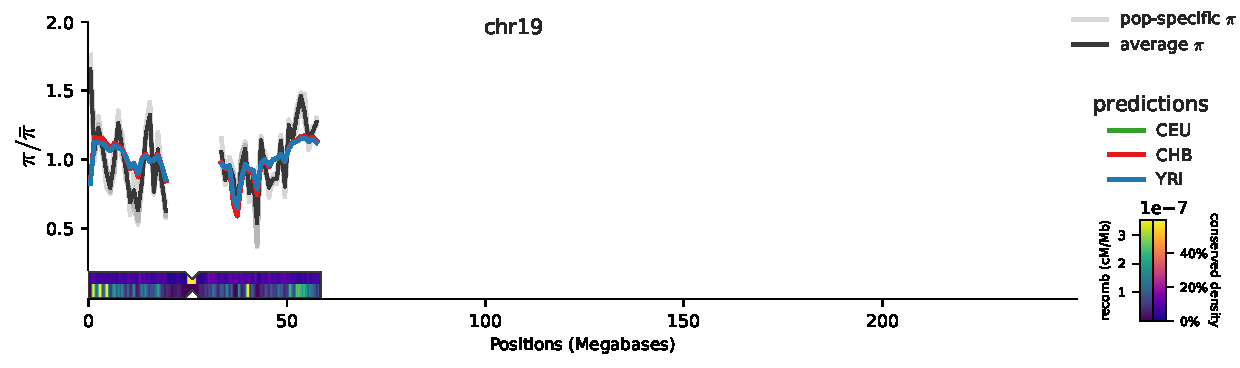
\includegraphics[width=\textwidth]{figures/supplementary/pred_plot_chr19.pdf}
  \label{suppfig:fit-chr19}
\end{figure}


\begin{figure}[!htb]
  \centering
  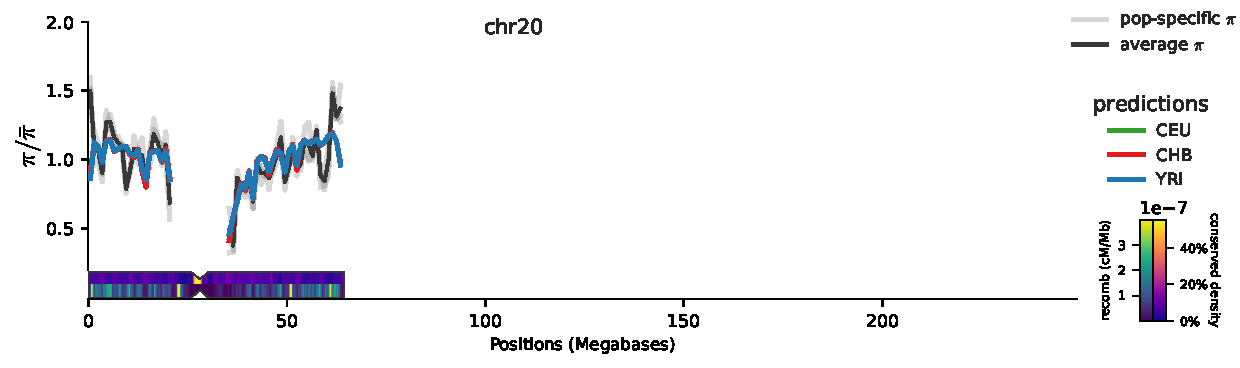
\includegraphics[width=\textwidth]{figures/supplementary/pred_plot_chr20.pdf}
  \label{suppfig:fit-chr20}
\end{figure}


\begin{figure}[!htb]
  \centering
  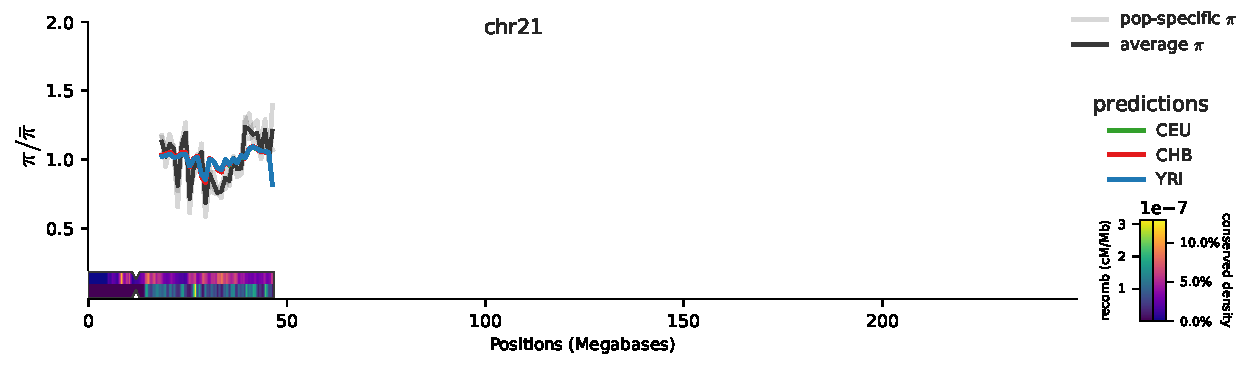
\includegraphics[width=\textwidth]{figures/supplementary/pred_plot_chr21.pdf}
  \label{suppfig:fit-chr21}
\end{figure}


\begin{figure}[!htb]
  \centering
  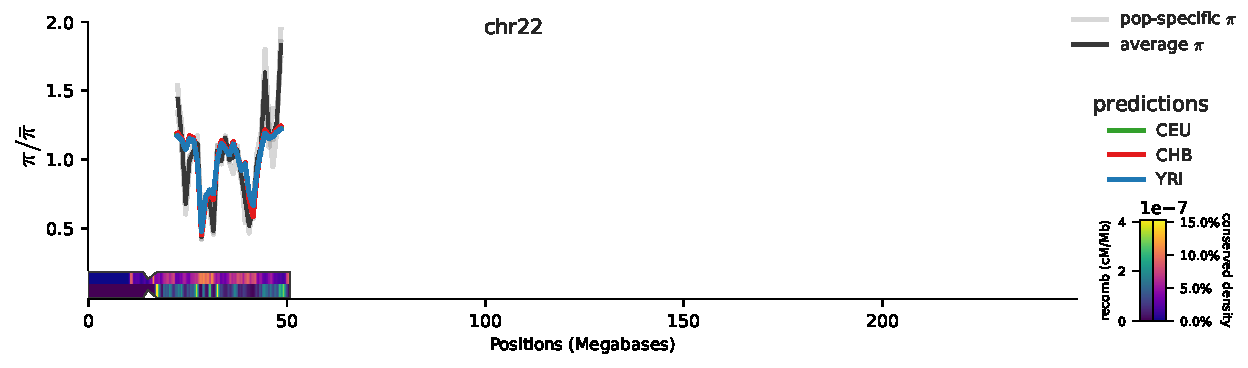
\includegraphics[width=\textwidth]{figures/supplementary/pred_plot_chr22.pdf}
  \label{suppfig:fit-chr22}
\end{figure}

\clearpage

%Our $B$ is,
%
%\begin{align}
%  B = \frac{1}{2N} \sum_{t=0}^\infty \prod_{i=0}^t \left(1 - \frac{1}{2N_e(i)}\right).
%\end{align}
%
%This sum takes many terms to converge, which makes calculating the $B$ between
%each focal neutral site and segment intractably slow (even when the equilibrium
%$\widetilde{V}$ for the segment pre-calculated). We approximate this in the
%following way for faster numerical calculations. Let $g(t) = \prod_{i=0}^t (1 -
%\nicefrac{1}{2N_e(i)})$. Then, taking the first-order series expansion around
%the logarithm of the terms and approximating the sum with an integral,
%
%\begin{align}
%  g(t) &\approx \exp\left(- \frac{1}{2N} \int_0^t \exp\left(\frac{V}{2} Q(x)^2 \right) dx \right) 
%       %&\approx \exp\left(- \int_0^t \frac{\exp\left(\frac{V}{2} Q(i)^2\right)}{2N}  dx \right)
%\end{align}
%
%$B$ is the case of $\lim b \to \infty$ for $B(b)$. Approximating the sum in
%$B(b)$ with an integral,
%
%\begin{align}
%  B(b) &= \int_0^b \exp\left(- \frac{1}{2N} \int_0^t \exp\left(\frac{V}{2} Q(x)^2 \right) dx \right) dt \\
%       %&\approx \exp\left(- \int_0^t \frac{\exp\left(\frac{V}{2} Q(i)^2\right)}{2N}  dx \right)
%\end{align}
%
%Now, let $z = \log(t)$, then
%
%\begin{align}
%  B(w) &= \int_0^w \exp\left(- \frac{1}{2N} \int_0^{\log(z)} \exp\left(\frac{V}{2} Q(x)^2 \right) dx \right) \exp(t) dz \\
%       %&\approx \exp\left(- \int_0^t \frac{\exp\left(\frac{V}{2} Q(i)^2\right)}{2N}  dx \right)
%\end{align}
%
%
\printbibliography

\end{document}
